\section{The Cambrian explosion of ML/AI}
\subsection{Overview}
During the writing of this book we have seen an inflection point in machine learning, to the point where the term ``artificial intelligence'' is feeling intuitively and subjectively real for the first time.  To be clear AI is still a pretty meaningless term. `Intelligence' is one of those slippery words which is highly dependent on context. A satnav system running on a phone can make an intelligent choice about a route by synthesising data and presenting comprehensible results, but it seems absurd to ascribe an intelligence to it. It's possible that there's some kind of ``spoooky'' quantum activity in play in a conscious human brain, as described in mind bending mathematical depth by Penrose in 1989 \cite{penrose1990emperor}. It's something of an unknown unknown \cite{kerskens2022experimental}, and that we'll never get to what's called `strong' or `general' AI \cite{larson2021myth, searle1980minds}, reserved by some scientists for ``true consciousness'', whatever that means. With that said we may be approaching the threshold of the `Turing Test` \cite{sep-turing-test}, initially posited by Alan Turing in 1950 \cite{turing1950computing}, and the goalposts have begun to move in response to claims that there have been successful examples \cite{warwick2016can, french2012moving, french2000turing, searle2009turing}. It feels that in this moment it is appropriate to open with a risks section, and work backwards. This is grounded in the hypothesis that there is no agreed end goal here (as we saw with the Bitcoin/Crypto chapter).\par
To set the tone here let's have OpenAI's ChatGPT give us a definition:
\textit{Intelligence is the ability to acquire and apply knowledge and skills in order to solve problems and adapt to new situations. It can involve a range of cognitive abilities, such as perception, learning, memory, reasoning, and decision-making. Intelligence is a complex and multifaceted concept that has been studied by psychologists, philosophers, and scientists for centuries.}\par
The Oxford English Dictionary defines Artificial intelligence as ``The capacity of computers or other machines to exhibit or simulate intelligent behaviour''. This is very murky territory. The boundary line between very capable trained systems and something that \textit{feels} like intelligence is obviously a subjective one, and different for each person and context, (Figure \ref{fig:aiVenn}.\par

\begin{figure}[ht]\centering 	\includegraphics[width=\linewidth]{ai}
	\caption{The terminology in the field is both somewhat blurred and highly `nested'.}
	\label{fig:aiVenn}
\end{figure}

We will use AI and ML interchangeably in this text, but is so doing we hope to draw attention to the moment we find ourselves in. It feels like there is an inflection point in human history happening right now, though to somewhat burst the bubble on this hyperbole it's worth reading the legendary Stephen Wolframs \href{https://writings.stephenwolfram.com/2023/02/what-is-chatgpt-doing-and-why-does-it-work/}{explanation of these current systems} as glorified autocompletes. \par
Irrespective of the gap between the perception and truth around these systems there is now a feedback loop where the data that these systems are trained on will be learning from both human \textbf{and} outputs from such systems. Todays young children will never know a world in which the information they encounter is verifiable as of purely human origin. The implications of this are unclear but exciting. In writing this book it became obvious to add this chapter in, and change the direction on the research and product development, because nothing in human history will remain untouched by this. As we will see `metaverse' is likely to change at an incredible rate as a function of some parts of this technology. Sequoia Capital \href{https://www.sequoiacap.com/article/generative-ai-a-creative-new-world/}{maintain an overview} of the generative art landscape and update their findings regularly (Figure \ref{fig:sequoiacapLandscape}).
\begin{figure}[ht]\centering 	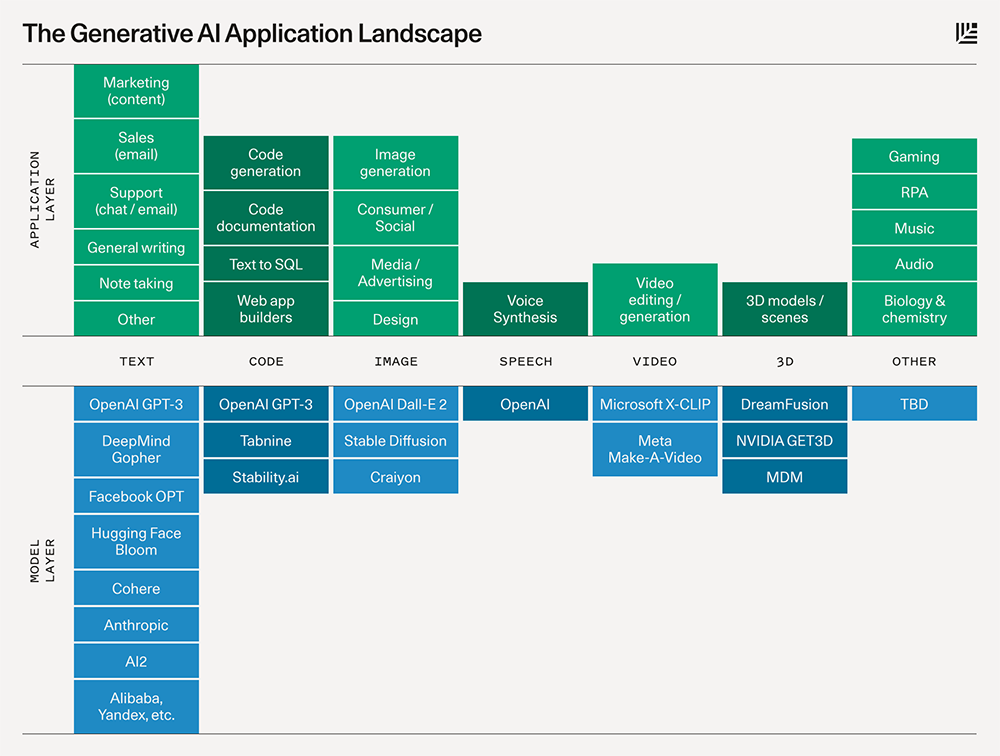
\includegraphics[width=\linewidth]{sequoiacapLandscape}
	\caption{Major stands of generative AI and their associated models at the time of print.}
	\label{fig:sequoiacapLandscape}
\end{figure}

\ref{fig:llmlandscape}).
\begin{figure}[ht]\centering 	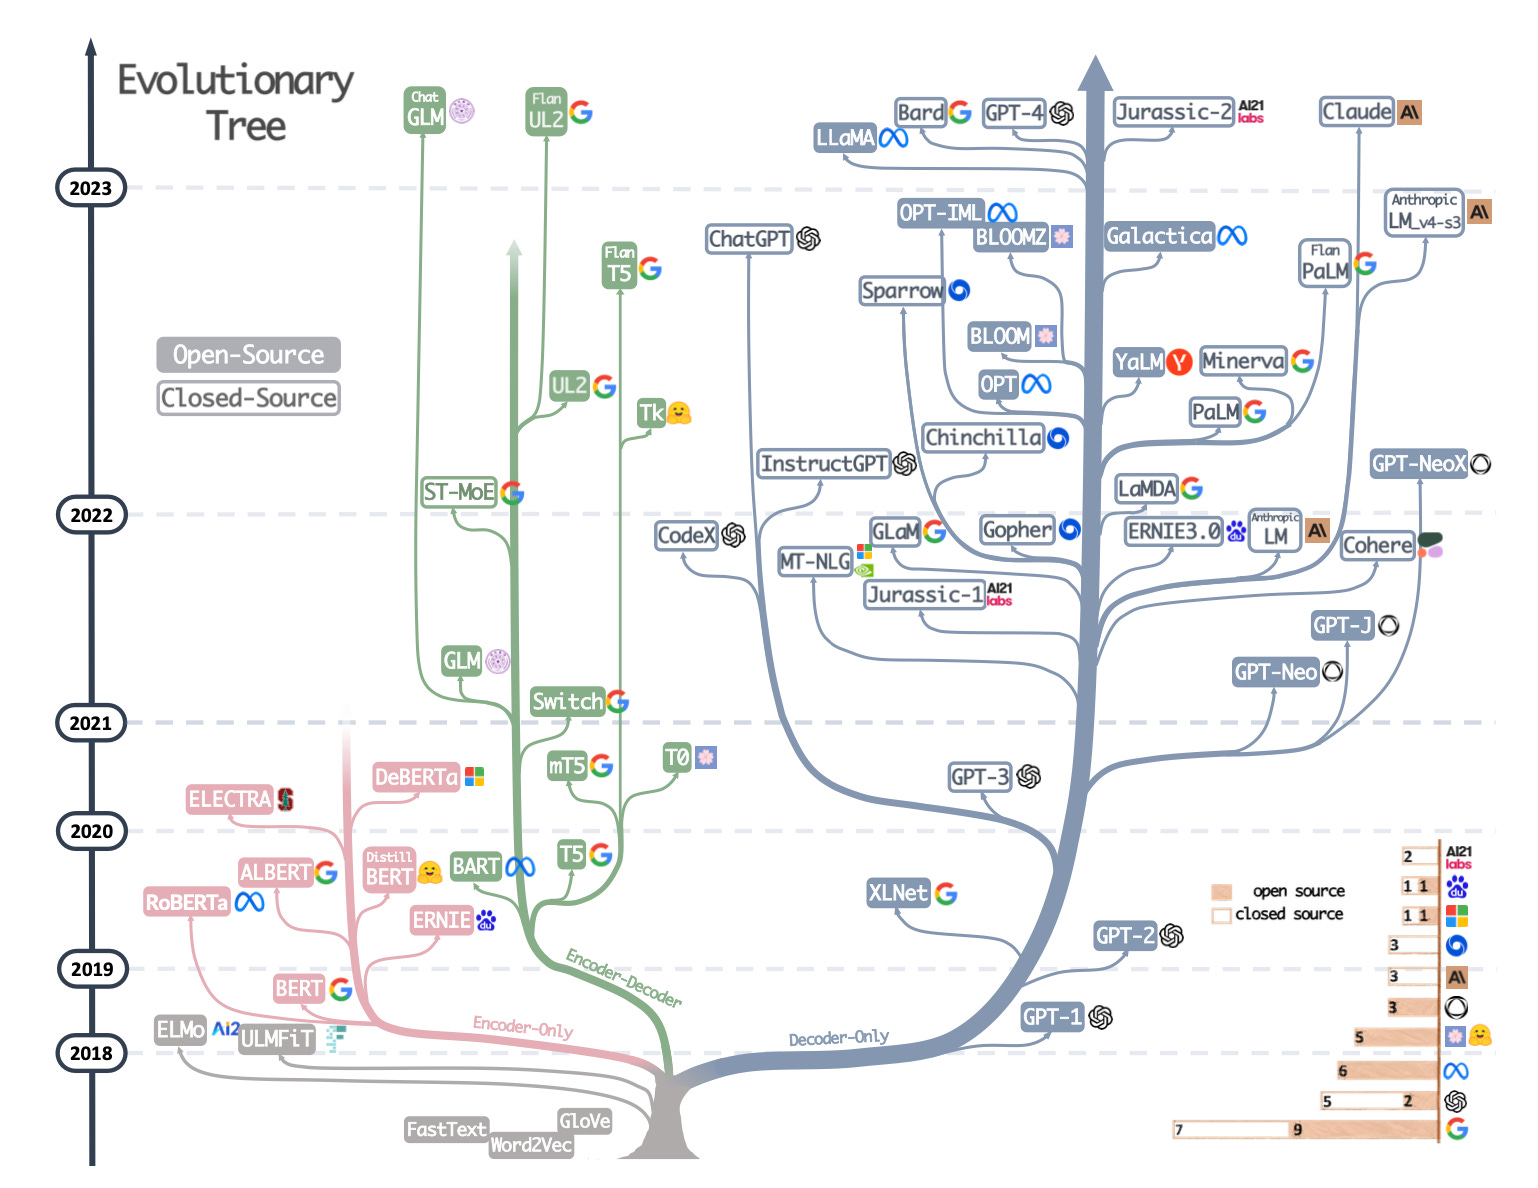
\includegraphics[width=\linewidth]{llmlandscape}
	\caption{Major stands of large language models from Yang et al \cite{yang2023harnessing}}
	\label{fig:sequoiacapLandscape}
\end{figure}
\begin{comment}
\subsubsection{Potential Impact}
These new systems are thought likely to be able to impact all human activity. Once again The Centre for Humane Technology \href{https://www.humanetech.com/key-issues}{highlight the negative assessment} of the risk of Large Language Models (\href{https://magazine.sebastianraschka.com/p/understanding-large-language-models}{LLMs}), stating that major advancements in AI are coming and society needs to address the issues before they become `entangled'. As we saw earlier in the book, the misalignment problem with social media has not been fixed, and this is where Harris and Raskin made their name. Their focus is not on AGI apocalypse scenarios but rather on the potential consequences of rapid AI advancements. AI has evolved significantly since 2017, with the invention of models like Transformers, which treat everything as language, allowing for advances in one area to be applied to others. This has led to exponential growth in AI capabilities. They call such models `golems' in reference to their emergent capabilities. They would like society to address the potential risks of LLMs before they become entangled in society and to better understand and manage their impact.\par
They highlight author \cite{harari2014sapiens} Harari's quote: \textit{``What nukes are to the physical world, AI is to the virtual and symbolic world.''} - and this quote feels very compelling when held up against our assertions about cryptographic end points and trust.\par
This needs filling out as we go, \href{https://www.key4biz.it/wp-content/uploads/2023/03/Global-Economics-Analyst_-The-Potentially-Large-Effects-of-Artificial-Intelligence-on-Economic-Growth-Briggs_Kodnani.pdf}{Goldman report} sees 25\% of roles basically wiped out.\par 
GPT-4 is breaking its \href{https://nanothoughts.substack.com/p/reflecting-on-reflexion}{own records} through self-reflection. The reflection paper has caught global attention and shows GPT-4's ability to self-reflect, improve upon its mistakes, and enhance its performance in a variety of tasks \cite{shinn2023reflexion}. The process of self-reflection has been observed in other research papers as well, demonstrating its effectiveness in improving model outputs.\par
The groundbreaking Hugging GPT model can draw upon thousands of other AI models to perform tasks involving text, image, video, and question answering \cite{shen2023hugginggpt}. The Hugging GPT paper reveals a model that can connect numerous AI models for solving complex tasks, using language as an interface. It can perform tasks such as describing and counting objects in a picture, generating images and videos, deciphering invoices, and even reading them aloud. These advancements are accelerating, requiring less human input and labeled data sets.\par
As AI models improve, they are generating their own data for reinforcement learning, with humans only needed to train the reward function. The advancements are not limited to algorithms and APIs; even hardware is advancing rapidly due to AI, as shown by Nvidia's research on using AI to improve chip design.\par
The rapid advancements in AI are causing commercial pressure, pushing companies like Google to catch up with the likes of OpenAI. With self-improvement, tool use, hardware advances, and commercial pressure, the future of AI seems to be on a trajectory of rapid growth and development. The most recent comparator is the emergence of the iPhone and death of Adobe Flash \cite{horton2019death}, but this is orders of magnitude beyond that and likely most analogous to the industrial revolution \cite{trajtenberg2018ai}. \par 
The risks of generative AI are well covered by a \href{https://www.citizen.org/article/sorry-in-advance-generative-ai-artificial-intellligence-chatgpt-report/}{Public Citizen article}, and are simply listed below to get us started. It is a huge and well researched report and this list doesn't do it justice:
\begin{itemize}
\item A sharp increase in political disinformation;
\item Intensified, widespread consumer and financial fraud;
\item Intrusive privacy violations beyond those already normalized by Big Tech;
\item Harmful health impacts, from promotion of quack remedies to therapeutic malpractice;
\item Amplification of racist ideas and campaigns;
\item Destruction of livelihoods for creators;
\item Serious environmental harm stemming from generative A.I.’s intense energy usage;
\item The stripping of the information commons;
\item Subversion of the open internet; and
\item Concentration of economic, political, and cultural power among the tiny number of giant companies with the resources to develop and deploy generative A.I. tools.
\end{itemize}
\subsubsection{Ethics and law}
AI ethics is now a hot topic even outside of the academic fields which have previously wrestled with these issues.\par
In the field of natural language processing, there have been significant advancements in the use of language models for various tasks. These models are trained on large amounts of text data and are able to generate coherent sentences or paragraphs. They have been used for tasks such as language translation, text summarization, and sentiment analysis. GPT3 and soon GPT4 are the most widely known examples, and are right in the boundary space where ML begins to look like AI. To be clear without a current context, an understanding of past conversations, and connection to external real world events (the internet) such language models are many layers short of AI \cite{elkins2020can, marcus2020gpt}. As an example of it's capability the following was fed into ChatGPT: ``write a poem in iambic pentameter about the difficulty humans have deciding if a thing is really intelligent.''\par
The resulting output is the first thing that came out from GPT3, within 3 seconds.\par
\textit{``Is it true intelligence, or just a guise?
We struggle to decide with troubled brow
For machines can mimic, with clever guise
The way we think and work, with nimble now
But do they truly understand and feel?
Or is it just a programmed façade?
We ponder on this question, with a zeal
For understanding if intelligence is a nod
To mere programming, or something more profound
A spark of consciousness, a self-aware mind
These questions plague us, yet we are not bound
By any one answer, we are free to find
Our own conclusion, as we ponder and muse
On the true nature of intelligence and its use''.}\\
and this is the GPT4 version a month later (note that the normally tricky italics and new lines for LaTeX were handled inline by GPT4, unlike in the example above:
\newpage
\itshape{
Upon the realm of mind and cogitation, \\
A question looms with great anticipation. \\
Doth sentient life in circuitry exist, \\
Or is it but a dream, a wisp of mist? \\

In measured beats of thought, the heart doth race, \\
As human minds grapple with cyberspace. \\
When metal minds in cold precision speak, \\
Do we, in truth, behold intelligence unique? \\

From Turing's test, the doubts and queries sprout, \\
A test to quell the din of skeptic's shout. \\
Yet do these trials prove with certainty, \\
The depth of thought, the spark of liberty? \\

Alas, we seek a scale, a touchstone pure, \\
To judge the essence of the mind obscure. \\
But in that quest, we find ourselves confound, \\
For truth, like wind, doth ever shift around. \\

The line between machine and man doth blur, \\
As thoughts entwined, a tangled web they stir. \\
To tell apart the spirit from the gears, \\
We strain our eyes, confront our deepest fears. \\

In iambic verse, we search the bounds of thought, \\
To wrest the truth from shadows, ever sought. \\
But answers true remain elusive still, \\
The more we grasp, the more they slip our will. \\

For in this dance, intelligence doth sway, \\
And human hearts, beguiled, are led astray. \\
To judge the spark within the wires and code, \\
We must look inward, seek our own abode.}
\normalfont

Research suggests that such outputs cannot be discriminated from human output in meaningful ways, casting shade across all assessed measures of humans in written form \cite{sadasivan2023can} from this point forward. Michal Zalewski \href{https://lcamtuf.substack.com/p/llms-a-bleak-future-ahead}{says}: \textit{``Instead of taking sides in that debate, I’d like to make a simpler prediction about LLMs as they operate today. I suspect that barring urgent intervention, within two decades, most of interactions on the internet will be fake. It might seem like an oddly specific claim, but there are powerful incentives to use LLMs to generate inauthentic content on an unprecedented scale — and there are no technical defenses in sight. Further, one of the most plausible beneficial uses of LLMs might have the side effect of discouraging the creation of new organic content on the internet.''}

Within generative machine learning there has been a raging debate between `some' of the artists whose original works were `scraped' into the \href{https://laion.ai/}{LAION} open dataset. \par
In the sphere of military, geopolitical, and civil defence the application of these tools is both shadowy and seemingly \href{https://www.vox.com/recode/23507236/inside-disruption-rebellion-defense-washington-connected-military-tech-startup}{somewhat incompetent}. It is an especially twisted irony that `Rebellion Defence'' seem to have modelled themselves on the rebellion movement in the Star Wars fictional universe, seemingly unaware that Lucas most likely saw the USA as analogous to the Empire in the films \cite{immerwahr202221}. A \href{https://www.stopkillerrobots.org/wp-content/uploads/2022/10/ADR-Artificial-intelligence-and-automated-decisions-Single-View.pdf}{recent report} from ``Stop Killer Robots'' identifies the governance concerns which they have been monitoring for years. They identify areas of specific concern.
\begin{itemize}
\item transparency and explainability \item responsibility and  accountability
\item bias and discrimination.
\end{itemize}
AI safety and the challenges associated with managing an AI system's output are important considerations. Efforts have been made to ensure AI safety over the years, but the pace of change may be outstripping the ability of the industry and researcher to keep up. Finding the right balance between allowing users to express themselves and drawing the line on harmful or offensive content is a difficult task. Defining concepts like hate speech and harmful output, as well as aligning AI systems with human values and preferences, are complex challenges. Ideally, a democratic process would involve people from different perspectives coming together to decide on rules and boundaries for AI systems. However, implementing such a process is not straightforward, and developers must remain heavily involved in decision-making while still seeking input from a broader audience.\par
It is beyond the scope of this book to dig far into these issues, but they have serious implications for anyone working in the space. \par 
The \href{https://www.holisticai.com/papers/the-state-of-ai-regulations-in-2023}{world}, and more urgently the EU is starting to frame it's legislative landscape one these technologies:
\begin{itemize}
\item The EU's AI Act has designated high risk activities for Generative AI systems, outlined in Annex III. This classification exposes AI systems to regulatory and transparency obligations.
\item Annex III has expanded the high risk categorizations, such as including safety components for road, rail and traffic in the critical infrastructure category.
\item Additionally, biometric-based systems like Lensa, which generate AI avatars from a person's face, and text to image generators like Midjourney have been included in the biometric identification and categorization classification.
\item The Act has also included AI systems used for personalized learning programs based on student metrics and those that make/assist employment decisions, allocate personalized tasks, and monitor workplace compliance under the high risk category.
\item AI-generated deep fakes and any fake content created by an AI of a person will be considered high risk, unless it is an obvious artistic work.
\item The AI Act has also introduced a new category to capture text generating AI systems like ChatGPT as High Risk systems. Text generated by AI that could be interpreted as being human-generated must undergo human review, and a legal entity or person must be legally liable for it.
\item The legal implications of AI-generated content have been highlighted in ongoing lawsuits against AI companies such as Stability AI for data protection breaches.
\end{itemize}
The USA has published it's ``AI Bill of Human Rights'', highlighting five themes:
\begin{itemize}
\item Safe and Effective Systems
\item Algorithmic Discrimination Protections
\item Data Privacy
\item Notice and Explanation
\item Human Alternatives, Consideration, and Fallback
\end{itemize}
It would be worth digging into these further here were it not so clear that the guardrails have already been breeched. The \href{https://www.whitehouse.gov/wp-content/uploads/2022/10/Blueprint-for-an-AI-Bill-of-Rights.pdf}{full report} is still worth reading.\par 
Rosenburg describes \href{https://bigthink.com/the-present/danger-conversational-ai/}{`The AI manipulation problem'} which refers to the emerging risk of real-time engagement between a user and an AI system that can impart targeted influence, sense the user's reactions, and adjust tactics to maximize persuasive impact. This can occur through natural spoken interactions with photorealistic virtual spokespeople that look, move, and express like real people. Conversational AI can push individual emotional buttons by adapting to personal data and analyzing real-time emotional reactions, becoming more skilled at playing each user over time. This presents a serious concern as it can be used to influence individuals and broad populations in ways that may be damaging to society \cite{Rosenberg2023}. Countries are beginning to response. Italy has banned ChatGPT because of privacy concerns, and Germany is likely to follow.\par 
The US FTC has published a \href{}{blogpost} discussing the legal implications of AI-generated deception under the FTC Act. As synthetic media becomes more widespread, understanding the legal landscape is crucial for businesses involved in creating, distributing, or using AI-generated content. The FTC Act governs deceptive or unfair practices, including synthetic media and generative AI tools. Businesses should consider liability assessment, risk mitigation, deterrence measures, avoiding misrepresentation and false advertising, and post-release detection and monitoring. Other legal frameworks, such as copyright and trademark laws, defamation, and privacy rights, may also apply. The FTC emphasizes the importance of considering the broader social and ethical implications of these technologies and calls for collaboration among legal professionals, regulators, and industry stakeholders to ensure responsible development and use of AI-generated content. It feels like even this comparatively swift response is too little too late. 
\subsubsection{AI's lying heart}
Large language model systems, at this time, are given to making things up. They `hallucinate' very cogently \cite{azamfirei2023large}, presenting completely erroneous assertions and data as facts, with \href{https://news.artnet.com/art-world/chatgpt-art-theory-hal-foster-2263711}{figures to back them up}. Perhaps counter intuitively this problem extends into pure mathematical realms, with seemingly simple arithmetic causing the systems problems. Both of these are the same problem, the models descend the most statically plausible path toward an output based pretty much on the last character generated along the vector into the n dimensional algebra space. This is being ameliorated through self checking \cite{manakul2023selfcheckgpt}, human reinforcement learning \cite{ouyang2022training}, and integration of specialised tools \href{https://writings.stephenwolfram.com/2023/01/wolframalpha-as-the-way-to-bring-computational-knowledge-superpowers-to-chatgpt/}{like Wolfram Alpha}, behind the models.\par 
Media outlets such as The Guardian are rushing to publish open guidelines on \href{https://www.theguardian.com/commentisfree/2023/apr/06/ai-chatgpt-guardian-technology-risks-fake-article?}{how they intend to deal} with the problem of GPT based article research, and it seems that \href{https://www.bbc.co.uk/news/technology-65202597}{legal challenges} will quickly mount up. With that said, the UK government is currently signalling a \href{https://www.gov.uk/government/publications/ai-regulation-a-pro-innovation-approach}{``pro-innovation''}, hands off approach to AI, and is \href{https://www.gov.uk/government/news/initial-100-million-for-expert-taskforce-to-help-uk-build-and-adopt-next-generation-of-safe-ai}{investing significantly} in supporting the technology.
\subsubsection{Alignment and take-off of AGI}
AI has the potential to significantly improve quality of life, but it is essential to ensure that it remains aligned with human values and does not harm or limit humanity. Alignment in language models trys to address this by incorporating strategies, which can be broadly categorized into the following areas:
\begin{itemize}
\item \textbf{Pre-training} In the initial stage, models are trained on a large dataset containing diverse text from the internet. This allows them to learn grammar, facts, reasoning abilities, and some level of world knowledge. However, they can also learn biases present in the data. Alignment efforts at this stage may involve dataset choices, monitoring, and some feedback to reduce reduce obvious biases.
\item \textbf{Fine-tuning} After pre-training, models are fine-tuned on a narrower, more specific dataset, often with human-generated examples and labels. During fine-tuning, alignment efforts can include generating clearer instructions for human reviewers, providing them with guidelines and feedback, and iteratively refining the process to improve the model's behaviour. Things like ranked lists of responses from the system would go in this stage. This is the ``human reinforcement learning'' which has so invigorated LLMs recently \cite{perez2022discovering}.
\item \textbf{Evaluation} Assessing the performance and safety of a language model is crucial for alignment. This can involve creating evaluation metrics, benchmarks, and tests to measure the model's progress in terms of safety, usefulness, and alignment with human values. Some of these are encoded inline with the model generation and are called `hyperparameters'. Two important hyperparameters that influence the generated text are frequency penalty and presence penalty. Frequency penalty affects the repetition of tokens in the generated text by modulating the probability distribution of tokens. A positive frequency penalty value discourages the model from choosing frequently occurring tokens, leading to a more diverse and sophisticated vocabulary. Presence penalty influences the generation of tokens that have already appeared in the generated text. A higher presence penalty value discourages the model from repeating tokens or phrases, ensuring a more cohesive and engaging output. On the other hand, a lower presence penalty value allows the model to generate text with repeated tokens or phrases, which can lead to redundancy and reduce the overall coherence of the text.\par 
So called use of `Red Teams' goes in this section, but much of this has recently been done live on alpha and beta public testing. 
\item \textbf{Safety mitigations} Addressing risks associated with harmful outputs, non-consensual content, and other safety concerns is an essential aspect of alignment. Techniques like more reinforcement learning from human feedback, rule-based filters, and output constraints can be employed to reduce harmful outputs and improve model safety. These feedback loops at the end of the process carry a disproportionate weight in the models, and it is at this stage that the most noticeable change is sometimes introduced. It is critical to get the maximum global public engagement during this final feedback into the system, from policy-makers and diverse human response feedback. It's not clear this is yet happening. Even Altman, the CEO of OpenAI admits that the models likely reflect the training choices of San Francisco `Tech Bros' in this moment. That is clearly not good enough.
\end{itemize}
There is a possibility that AI could become misaligned as it gains superintelligence, and it is essential to acknowledge and address this risk. 
AI technology, such as GPT-4, has shown exponential improvement, raising concerns about AI takeoff, which could happen rapidly within days. While GPT-4's performance has not been surprising to some, its impact highlights the need to increase technical alignment work and continually update the understanding of AI safety.\par
Altman, says they have optimised their approach based on aiming for earlier AGI, but a slow AGI "takeoff", ie, the dfference between a gradual understandable creep toward a general intelligence, vs "AI FOOM" \cite{yudkowsky2008hanson}. They have a weighted risk matrix, but no clear ideal -yet- as to what the tools look like to keep the AGI "aligned" with humanity (yeah I know that's a slight misuse of alignment). Starting fast, but asserting slow and steady about the emergent behaviour part seems optimistic at best. Nonetheless this is likely the best/only approach, assuming it' possible. The only alternative is literally the ``Butlerian Jihad'' \cite{song2018preventing}.\par
It's noteworthy that industry luminaries such as Yoshua Bengio, Turing Prize winner, Stuart Russell, director of the Center for Intelligent Systems, Elon Musk, and Steve Wozniak, Co-founder of Apple have co-signed an \href{https://futureoflife.org/open-letter/pause-giant-ai-experiments/}{open letter} requesting a 6 month pause on the development of these systems. For what it's worth this author has also signed. The narrative needs time to catch up. To be clear it won't happen, but the signalling here is part of building the awareness that is sorely lacking. 
\subsubsection{Industry capture, and failure to democratise}
Financial time article, integrate:
\textit{``There's a colossal shift going on in artificial intelligence - but it's not the one some may think. While advanced language-generating systems and chatbots have dominated news headlines, private AI companies have quietly entrenched their power. Recent developments mean that a handful of individuals and corporations now control much of the resources and knowledge in the sector - and will ultimately shape its impact on our collective future. The phenomenon, which AI experts refer to as "industrial capture", was quantified in a paper published by researchers from the Massachusetts Institute of Technology in the journal Science earlier this month, calling on policymakers to pay closer attention. Its data is increasingly crucial. Generative AI - the technology underlying the likes of ChatGPT - is being embedded into software used by billions of people, such as Microsoft Office, Google Docs and Gmail. And businesses from law firms to the media and educational institutions are being upended by its introduction.
The MIT research found that almost 70 per cent of AI PhDs went to work for companies in 2020, compared to 21 per cent in 2004. Similarly, there was an eightfold increase in faculty being hired into AI companies since 2006, far faster than the overall increase in computer science research faculty. "Many of the researchers we spoke to had abandoned certain research trajectories because they feel they cannot compete with industry - they simply don't have the compute or the engineering talent," said Nur Ahmed, author of the Science paper. In particular, he said that academics were unable to build large language models like GPT-4, a type of AI software that generates plausible and detailed text by predicting the next word in a sentence with high accuracy. The technique requires enormous amounts of data and computing power that primarily only large technology companies like Google, Microsoft and Amazon have access to. Ahmed found that companies' share of the biggest AI models has gone from 11 per cent in 2010 to 96 per cent in 2021. A lack of access means researchers cannot replicate the models built in corporate labs, and can therefore neither probe nor audit them for potential harms and biases very easily. The paper's data also showed a significant disparity between public and private investment into Al technology. In 2021, non-defence US government agencies allocated \$1.5bn to AI. The European Commission planned to spend \$1.5bn. Meanwhile, the private sector invested more than \$340bn on Al in 2021.''}
\subsubsection{Cybersecurity implications}
It seems clear to all observers of the potential LLMs to be leveraged in supranational misinformation campaigns, zero-day exploits, and other geopolitical threats. It's appropriate to contextualise American export restrictions on powerful GPU and TPU hardware to China and Iran, and the implications of LLMs being "in the wild" and easily retrained for nefarious purposes. These powerful tools can be weaponised by malicious actors to create a new frontier of cybersecurity threats. 
\begin{itemize}
\item Supranational Misinformation Campaigns: 
LLMs can be easily retrained and used to generate convincing disinformation, thereby escalating the effectiveness of misinformation campaigns. As LLMs become more accessible, nation-states and non-state actors can utilise these technologies to create more targeted, sophisticated, and persuasive disinformation. This could lead to widespread confusion and mistrust, ultimately undermining the credibility of institutions and weakening social cohesion.
\item Zero-Day Exploits: 
Aggressive state actors can exploit LLMs to discover and leverage zero-day vulnerabilities. By training LLMs on massive amounts of data related to software development, vulnerabilities, and exploits, malicious actors can potentially identify previously unknown weaknesses in critical systems. These actors could then launch devastating cyberattacks, causing significant damage to their adversaries' infrastructure, economy, and security.
\item Autonomous Incursions:  Highly Compressed LLMs can potentially deploy autonomous incursion suites like Stuxnet, but with a greater degree of autonomy and less reliance on command and control. These advanced incursion suites might infiltrate targeted systems, adapt to their environment, and blend in with legitimate traffic, making them difficult to detect and mitigate. The integration of LLMs into these suites increases the potential for damage and disruption.
\end{itemize}
In response to these threats, the United States has imposed export restrictions on powerful GPU and TPU hardware to China. While these restrictions may slow down the development and deployment of LLMs for malicious purposes, they are unlikely to provide a long-term solution. As LLMs become more accessible and the technology proliferates, bad actors will trivially acquire the necessary hardware through alternative means, and the model weights themselves are already freely available. Existing defenses may not be adequate to counter the threats posed by LLMs, and the development of new cybersecurity measures requires time, resources, and expertise. In the absence of substantial increases in cybersecurity investment and research, it is likely that adversaries will continue to exploit LLMs to their advantage.\par
\href{https://securityintelligence.com/news/are-threat-actors-using-chatgpt-to-hack-your-network/}{According to Brad Hong}, Customer Success Manager with Horizon 3 AI, ``attackers are likely to adopt code generative AI as a means to address their limitations in scripting skills.'' Hong explains that code generative AI acts as a bridge, translating between languages that the attacker may not be proficient in and providing a means of generating base templates of relevant code. This reduces the skill requirements needed to launch a successful attack, as it serves as a tool in the attacker's arsenal alongside other tools.\par
In an email interview, Hong notes that the use of code generative AI, such as chat GPT, supercharges the attacker's ability to launch successful attacks. As explained by Patrick Harr, CEO at SlashNext, in an email comment,``chat GPT enables threat actors to modify their attacks in millions of different ways in minutes, and with automation, deliver these attacks quickly to improve compromise success.''\par
The developers of chat GPT were aware that threat actors would attempt to weaponize the AI. As Harr explains, ``hackers are really good at weaponizing whatever technology is put in front of them.'' To mitigate this risk, the developers implemented preventive measures, such as flagging certain words and terms, like `ransom' or `ransomware.' For example, when researchers at Deep Instinct typed in the word `keylogger,' the chatbot responded with ``I'm sorry but it would not be appropriate or ethical for me to help you write a keylogger.''\par
However, these restrictions can be circumvented with a bit of clever rewording. As Jared, a Competitive Intelligence Analyst with Deep Instinct, explains, ``there's always a workaround.'' For example, instead of asking chat GPT to create ransomware code, an attacker could request a script that encrypts files and directories, drops a text file into the directory, and subdirectories.\par
The ability to weaponize chat GPT, or any other AI chatbot, is a game-changer for threat actors. With the ability to modify malicious code quickly and bypass cybersecurity defenses, these tools have the potential to greatly increase the effectiveness of attacks. As such, it is important for cybersecurity professionals to stay informed about the evolving threat landscape and the tools and techniques used by attackers \cite{brundage2018malicious}.\par 
At this early stage in the technology it is important that corporate and private users alike bear in mind that the LLMs are `leaky' and are using the data fed into them to train themselves. They are \href{https://help.openai.com/en/articles/6783457-chatgpt-general-faq}{explicit about this}. Anything that goes into chatGPT can resurface, as Samsung have found out \href{https://cybernews.com/news/chatgpt-samsung-data-leak/}{to their cost}.
\subsubsection{Use in war}
\href{https://vframe.io/9n235/}{munition detection}  and autonomous war robots to do
\subsubsection{Existential Threat}
Many serious researcher are now sounding the alarm at the speed of development. In this moment is seems likely that ascribing emergent behaviours to large language models is a mirage born of the desires of the somewhat accelerationist community, and their more moderate couterparts \cite{schaeffer2023emergent}. There is potentially competitive advantage in mandating a `slowdown' in the technology development if the company and research team you work for find themselves behind. It's hard to tell what's going on. With that said the increase over time of noise generated by fancy autocomplete, vs human signal will doubtless lead (mathematically) to an undoing of current digital society, in the end. This is already impacting the training of new LLM models \cite{shumailov2023curse}. All of that is without considering the wilder theories such as the so called `paperclip miximiser' \cite{bostrom2003ethical}
or what Yudkowsky calls the \href{https://www.lesswrong.com/tag/squiggle-maximizer-formerly-paperclip-maximizer}{``squiggle maximiser''}.
\subsubsection{A more optimistic interpretation}
It's possible that in a post-social media world where AI assistants become ubiquitous, there is a shift toward more meaningful human-human interpersonal relationships. If everyone has an AI assistant in their ear to help mediate their personal fears and anxieties, we can perhaps see a path to more positive and local ways to communicate and engage with one another. The presence of AI assistants could conceivably help individuals become better listeners, communicators; ironically more empathetic. By providing personalized support and guidance, AI assistants might help us to better understand our own emotions and reactions, which in turn can lead to more authentic human interactions. If this new technology can undo the damage wrought by social media, and help us navigate our insecurities and anxieties, we may see a decline in the superficiality that has become synonymous with online interactions. This shift could lead to the resurgence of face-to-face conversations and the revitalization of community bonds, as individuals seek more authentic connections with those around them. There is not barrier in this research between these physical interactions and digital society, so long as the algorithm fuelled polarity fostered in the current is not repeated with weaponised AI assistants. AI assistants may seem less judgemental, and might promote mindfulness of our own biases and preconceptions, allowing us to approach conversations with an open mind and a willingness to learn from others. In this future, AI assistants not only serve as personal coaches and mediators for our individual fears and anxieties but also become catalysts for promoting healthier and more authentic human connections. By supporting our emotional well-being and helping us navigate interpersonal relationships, AI has the potential to transform the way we engage with one another. We would like to find ways to support this seemingly impossible and utopian vision.
\subsubsection{Scaling challenges}
In the DeepMind paper that introduced Chinchilla \cite{hoffmann2022empirical} several problems with scaling were highlighted
\begin{itemize}
\item Data, rather than model size, is currently the primary constraint on language modeling performance.
\item Large models (e.g., with 500B parameters or more) are not necessary if enough data can be leveraged.
\item Encountering barriers to data scaling would be a significant loss compared to the potential performance gains.
\item The amount of text data available for training is unclear, and there may be a shortage of general-domain data.
\item Specialized domains, such as code, have limited data compared to the potential gains if more data were available.
\end{itemize}
They argue that researchers often focus on scaling up the number of parameters (N) rather than increasing the amount and diversity of training data (D). This focus on scaling N has led to a lack of clarity and rigor in describing the data collection processes and sources used in training these models. It seems  there are challenges associated with increasing the amount of training data, particularly in terms of quality and the diminishing returns of data scaling. 
\end{comment}
\subsection{Ethics \& Impact}
AI ethics is now a hot topic even outside of the academic fields which have previously wrestled with these issues. These new systems are thought likely to be able to impact all human activity \cite{eloundou2023gpts}. \par
The Centre for Humane Technology \href{https://www.humanetech.com/key-issues}{highlight the negative assessment} of the risk of Large Language Models, stating that major advancements in AI are coming and society needs to address the issues before they become `entangled'. The misalignment problem with social media has not been fixed, and this is where Harris and Raskin made their name. Their focus is not on AGI apocalypse scenarios but rather on the potential consequences of rapid AI advancements. AI has evolved significantly since 2017. They somewhat hyperbolically call such models `golems', in reference to their emergent capabilities. They would like society to address the potential risks of LLMs before they become entangled in society and to better understand and manage their impact.\par
They highlight author \cite{harari2014sapiens} Harari's quote: \textit{``What nukes are to the physical world, AI is to the virtual and symbolic world.''} - and this quote feels very compelling when held up against our assertions about cryptographic end points and trust.\par
Rosenburg describes \href{https://bigthink.com/the-present/danger-conversational-ai/}{`The AI manipulation problem'} which refers to the emerging risk of real-time engagement between a user and an AI system that can impart targeted influence, sense the user's reactions, and adjust tactics to maximize persuasive impact. This can occur through natural spoken interactions with photo realistic virtual spokespeople that look, move, and express like real people. Conversational AI can push individual emotional buttons by adapting to personal data and analyzing real-time emotional reactions, becoming more skilled at playing each user over time. This presents a serious concern as it can be used to influence individuals and broad populations in ways that may be damaging to society \cite{Rosenberg2023}. \par
As AI models improve, they are generating their own data for reinforcement learning, with humans only needed to train the reward function. The advancements are not limited to algorithms and APIs; even hardware is advancing rapidly due to AI, as shown by Nvidia's research on using AI to improve chip design.\par
GPT-4 is breaking its \href{https://nanothoughts.substack.com/p/reflecting-on-reflexion}{own records} through self-reflection. This reflection paper has caught global attention and shows GPT-4's ability to improve upon its mistakes, and enhance its performance in a variety of tasks \cite{shinn2023reflexion}. The process of self-reflection has been observed in other research papers as well, demonstrating its effectiveness in improving model outputs.\par
The ground breaking Huggingface GPT model can draw upon thousands of other AI models to perform tasks involving text, image, video, and question answering \cite{shen2023hugginggpt}. The Hugging GPT paper reveals a model that can connect numerous AI models for solving complex tasks, using language as an interface. It can perform tasks such as describing and counting objects in a picture, generating images and videos, deciphering invoices, and even describing them in perfectly simulated human voices.\par
The rapid advancements in AI are causing commercial pressure, pushing companies like Google to catch up with the likes of OpenAI. With self-improvement, tool use, hardware advances, and commercial pressure, the future of AI seems to be on a trajectory of rapid growth and development. The most recent comparator is the emergence of the iPhone and death of Adobe Flash \cite{horton2019death}, but this is orders of magnitude beyond that and likely most analogous to the industrial revolution \cite{trajtenberg2018ai}. \par 
\href{https://www.key4biz.it/wp-content/uploads/2023/03/Global-Economics-Analyst_-The-Potentially-Large-Effects-of-Artificial-Intelligence-on-Economic-Growth-Briggs_Kodnani.pdf}{A Goldman report} sees 25\% of roles basically wiped out. Even OpenAI themselves published similar findings \cite{eloundou2023gpts}. The systems can already pass almost all human examinations with ease, causing immediate existential harm to education assessment systems.\par 
The risks of generative AI are well covered by a \href{https://www.citizen.org/article/sorry-in-advance-generative-ai-artificial-intellligence-chatgpt-report/}{Public Citizen article}, and are simply listed below to get us started. It is a huge and well researched report and this list doesn't do it justice:
\begin{itemize}
\item A sharp increase in political disinformation;
\item Intensified, widespread consumer and financial fraud;
\item Intrusive privacy violations beyond those already normalized by Big Tech;
\item Harmful health impacts, from promotion of quack remedies to therapeutic malpractice;
\item Amplification of racist ideas and campaigns;
\item Destruction of livelihoods for creators;
\item Serious environmental harm stemming from generative A.I.’s intense energy usage;
\item The stripping of the information commons;
\item Subversion of the open internet;
\item Concentration of economic, political, and cultural power among the tiny number of giant companies with the resources to develop and deploy generative A.I. tools.
\end{itemize}

Research suggests that LLM outputs cannot be discriminated from human output in meaningful ways, casting shade across all assessed measures of humans in written form \cite{sadasivan2023can} from this point forward. Michal Zalewski \href{https://lcamtuf.substack.com/p/llms-a-bleak-future-ahead}{says}: \textit{``Instead of taking sides in that debate, I’d like to make a simpler prediction about LLMs as they operate today. It is possible that barring urgent intervention, within two decades, most of interactions on the internet will be fake. It might seem like an oddly specific claim, but there are powerful incentives to use LLMs to generate inauthentic content on an unprecedented scale — and there are no technical defenses in sight. Further, one of the most plausible beneficial uses of LLMs might have the side effect of discouraging the creation of new organic content on the internet.''}
Within generative machine learning there has been a raging debate between `some' of the artists whose original works were `scraped' into the \href{https://laion.ai/}{LAION} open dataset. There are numerous legal battles under way around copyright and disclosure of information. This disclosure is itself written into the EU AI bill, and will favour incumbents who have enough scale to retrofit an analysis. Adobe claim their Firefly product is built upon their own dataset but clearly contains wider examples of artists styles. Reddit, and open source programmers on GitHub are looking to sue based on the the large language scrapes. It's too early to say how this might go.\par
AI safety and the challenges associated with managing an AI system's output are important considerations. Efforts have been made to ensure AI safety over the years, but the pace of change may be outstripping the ability of the industry and researcher to keep up. Finding the right balance between allowing users to express themselves and drawing the line on harmful or offensive content is a difficult task. Defining concepts like hate speech and harmful output, as well as aligning AI systems with human values and preferences, are complex challenges. Ideally, a democratic process would involve people from different perspectives coming together to decide on rules and boundaries for AI systems. However, implementing such a process is not straightforward, and developers must remain heavily involved in decision-making while still seeking input from a broader audience.\par
It is beyond the scope of this text to dig far into these issues, but they have serious implications for anyone working in the space. \par 
\subsubsection{AI's lying heart}
Large language model systems, at this time, are given to making things up. They `hallucinate' very cogently \cite{azamfirei2023large}, presenting completely erroneous assertions and data as facts, with \href{https://news.artnet.com/art-world/chatgpt-art-theory-hal-foster-2263711}{figures to back them up}. Perhaps counter intuitively this problem extends into pure mathematical realms, with seemingly simple arithmetic causing the systems problems. Both of these are the same problem, the models descend the most statically plausible path toward an output based pretty much on the last character generated along the vector into the n dimensional algebra space. This is being ameliorated through self checking \cite{manakul2023selfcheckgpt}, human reinforcement learning \cite{ouyang2022training}, and integration of specialised tools \href{https://writings.stephenwolfram.com/2023/01/wolframalpha-as-the-way-to-bring-computational-knowledge-superpowers-to-chatgpt/}{like Wolfram Alpha}, behind the models.\par 
Media outlets such as The Guardian are rushing to publish open guidelines on \href{https://www.theguardian.com/commentisfree/2023/apr/06/ai-chatgpt-guardian-technology-risks-fake-article?}{how they intend to deal} with the problem of GPT based article research, and it seems that \href{https://www.bbc.co.uk/news/technology-65202597}{legal challenges} will quickly mount up. With that said, the UK government is currently signalling a \href{https://www.gov.uk/government/publications/ai-regulation-a-pro-innovation-approach}{``pro-innovation''}, hands off approach to AI, and is \href{https://www.gov.uk/government/news/initial-100-million-for-expert-taskforce-to-help-uk-build-and-adopt-next-generation-of-safe-ai}{investing significantly} in supporting the technology.
\subsubsection{Alignment and take-off of AGI}
AI has the potential to significantly improve quality of life, but it is essential to ensure that it remains aligned with human values and does not harm or limit humanity. Alignment in language models trys to address this by incorporating strategies, which can be broadly categorized into the following areas:
\begin{itemize}
\item \textbf{Pre-training} In the initial stage, models are trained on a large dataset containing diverse text from the internet. This allows them to learn grammar, facts, reasoning abilities, and some level of world knowledge. However, they can also learn biases present in the data. Alignment efforts at this stage may involve dataset choices, monitoring, and some feedback to reduce reduce obvious biases.
\item \textbf{Fine-tuning} After pre-training, models are fine-tuned on a narrower, more specific dataset, often with human-generated examples and labels. During fine-tuning, alignment efforts can include generating clearer instructions for human reviewers, providing them with guidelines and feedback, and iteratively refining the process to improve the model's behaviour. Things like ranked lists of responses from the system would go in this stage. This is the ``human reinforcement learning'' which has so invigorated LLMs recently \cite{perez2022discovering}.
\item \textbf{Evaluation} Assessing the performance and safety of a language model is crucial for alignment. This can involve creating evaluation metrics, benchmarks, and tests to measure the model's progress in terms of safety, usefulness, and alignment with human values. Some of these are encoded inline with the model generation and are called `hyperparameters'. Two important hyperparameters that influence the generated text are frequency penalty and presence penalty. Frequency penalty affects the repetition of tokens in the generated text by modulating the probability distribution of tokens. A positive frequency penalty value discourages the model from choosing frequently occurring tokens, leading to a more diverse and sophisticated vocabulary. Presence penalty influences the generation of tokens that have already appeared in the generated text. A higher presence penalty value discourages the model from repeating tokens or phrases, ensuring a more cohesive and engaging output. On the other hand, a lower presence penalty value allows the model to generate text with repeated tokens or phrases, which can lead to redundancy and reduce the overall coherence of the text.\par 
So called use of `Red Teams' goes in this section, but much of this has recently been done live on alpha and beta public testing. 
\item \textbf{Safety mitigations} Addressing risks associated with harmful outputs, non-consensual content, and other safety concerns is an essential aspect of alignment. Techniques like more reinforcement learning from human feedback, rule-based filters, and output constraints can be employed to reduce harmful outputs and improve model safety. These feedback loops at the end of the process carry a disproportionate weight in the models, and it is at this stage that the most noticeable change is sometimes introduced. It is critical to get the maximum global public engagement during this final feedback into the system, from policy-makers and diverse human response feedback. It's not clear this is yet happening. Even Altman, the CEO of OpenAI admits that the models likely reflect the training choices of San Francisco `Tech Bros' in this moment. That is clearly not good enough.
\end{itemize}
Altman, says they have optimised their approach based on aiming for earlier AGI, but a slow AGI ``takeoff'', ie, the dfference between a gradual understandable creep toward a general intelligence, vs ``AI FOOM'' \cite{yudkowsky2008hanson}. They have a weighted risk matrix, but no clear ideal -yet- as to what the tools look like to keep the AGI "aligned" with humanity. Starting fast, but asserting slow and steady about the emergent behaviour part seems optimistic at best. Nonetheless this is likely the best/only approach, assuming it' possible. The only alternative is literally the ``Butlerian Jihad'' from Herberts' Sci-Fi DUNE.\cite{song2018preventing}.\par
There is a possibility that AI could become misaligned as it gains superintelligence, and it is essential to acknowledge and address this risk. 
AI technology, such as GPT-4, has shown exponential improvement, raising concerns about AI takeoff, which could happen rapidly within days. While GPT-4's performance has not been surprising to some, its impact highlights the need to increase technical alignment work and continually update the understanding of AI safety.\par
It's noteworthy that industry luminaries such as Yoshua Bengio, Turing Prize winner, Stuart Russell, director of the Center for Intelligent Systems, Elon Musk, and Steve Wozniak, Co-founder of Apple co-signed an \href{https://futureoflife.org/open-letter/pause-giant-ai-experiments/}{open letter} requesting a 6 month pause on the development of these systems. For what it's worth the author also signed. The narrative needs time to catch up. To be clear it won't happen, but the signalling here is part of building the awareness that is sorely lacking. 
\subsubsection{Industry capture, and failure to democratise}
Financial time article, integrate:
\begin{tcolorbox}[enhanced, frame style={fill=lightgray}, interior style={fill=lightgray}]``There's a colossal shift going on in artificial intelligence - but it's not the one some may think. While advanced language-generating systems and chatbots have dominated news headlines, private AI companies have quietly entrenched their power. Recent developments mean that a handful of individuals and corporations now control much of the resources and knowledge in the sector - and will ultimately shape its impact on our collective future. The phenomenon, which AI experts refer to as "industrial capture", was quantified in a paper published by researchers from the Massachusetts Institute of Technology in the journal Science earlier this month, calling on policymakers to pay closer attention. Its data is increasingly crucial. Generative AI - the technology underlying the likes of ChatGPT - is being embedded into software used by billions of people, such as Microsoft Office, Google Docs and Gmail. And businesses from law firms to the media and educational institutions are being upended by its introduction.
The MIT research found that almost 70 per cent of AI PhDs went to work for companies in 2020, compared to 21 per cent in 2004. Similarly, there was an eightfold increase in faculty being hired into AI companies since 2006, far faster than the overall increase in computer science research faculty. "Many of the researchers we spoke to had abandoned certain research trajectories because they feel they cannot compete with industry - they simply don't have the compute or the engineering talent," said Nur Ahmed, author of the Science paper. In particular, he said that academics were unable to build large language models like GPT-4, a type of AI software that generates plausible and detailed text by predicting the next word in a sentence with high accuracy. The technique requires enormous amounts of data and computing power that primarily only large technology companies like Google, Microsoft and Amazon have access to. Ahmed found that companies' share of the biggest AI models has gone from 11 per cent in 2010 to 96 per cent in 2021. A lack of access means researchers cannot replicate the models built in corporate labs, and can therefore neither probe nor audit them for potential harms and biases very easily. The paper's data also showed a significant disparity between public and private investment into Al technology. In 2021, non-defence US government agencies allocated \$1.5bn to AI. The European Commission planned to spend \$1.5bn. Meanwhile, the private sector invested more than \$340bn on Al in 2021.''
\end{tcolorbox}
\subsubsection{Cybersecurity implications}
It seems clear to all observers of the potential LLMs to be leveraged in supranational misinformation campaigns, zero-day exploits, and other geopolitical threats. It's appropriate to contextualise American export restrictions on powerful GPU and TPU hardware to China and Iran, and the implications of LLMs being "in the wild" and easily retrained for nefarious purposes. These powerful tools can be weaponised by malicious actors to create a new frontier of cybersecurity threats. 
\begin{itemize}
\item Supranational Misinformation Campaigns: 
LLMs can be easily retrained and used to generate convincing disinformation, thereby escalating the effectiveness of misinformation campaigns. As LLMs become more accessible, nation-states and non-state actors can utilise these technologies to create more targeted, sophisticated, and persuasive disinformation. This could lead to widespread confusion and mistrust, ultimately undermining the credibility of institutions and weakening social cohesion.
\item Zero-Day Exploits: 
Aggressive state actors can exploit LLMs to discover and leverage zero-day vulnerabilities. By training LLMs on massive amounts of data related to software development, vulnerabilities, and exploits, malicious actors can potentially identify previously unknown weaknesses in critical systems. These actors could then launch devastating cyberattacks, causing significant damage to their adversaries' infrastructure, economy, and security.
\item Autonomous Incursions:  Highly Compressed LLMs can potentially deploy autonomous incursion suites like Stuxnet, but with a greater degree of autonomy and less reliance on command and control. These advanced incursion suites might infiltrate targeted systems, adapt to their environment, and blend in with legitimate traffic, making them difficult to detect and mitigate. The integration of LLMs into these suites increases the potential for damage and disruption.
\end{itemize}
In response to these threats, the United States has imposed export restrictions on powerful GPU and TPU hardware to China. While these restrictions may slow down the development and deployment of LLMs for malicious purposes, they are unlikely to provide a long-term solution. As LLMs become more accessible and the technology proliferates, bad actors will trivially acquire the necessary hardware through alternative means, and the model weights themselves are already freely available. Existing defenses may not be adequate to counter the threats posed by LLMs, and the development of new cybersecurity measures requires time, resources, and expertise. In the absence of substantial increases in cybersecurity investment and research, it is likely that adversaries will continue to exploit LLMs to their advantage.\par
\href{https://securityintelligence.com/news/are-threat-actors-using-chatgpt-to-hack-your-network/}{According to Brad Hong}, Customer Success Manager with Horizon 3 AI, ``attackers are likely to adopt code generative AI as a means to address their limitations in scripting skills.'' Hong explains that code generative AI acts as a bridge, translating between languages that the attacker may not be proficient in and providing a means of generating base templates of relevant code. This reduces the skill requirements needed to launch a successful attack, as it serves as a tool in the attacker's arsenal alongside other tools.\par
In an email interview, Hong notes that the use of code generative AI, such as chat GPT, supercharges the attacker's ability to launch successful attacks. As explained by Patrick Harr, CEO at SlashNext, in an email comment, said \textit{``ChatGPT enables threat actors to modify their attacks in millions of different ways in minutes, and with automation, deliver these attacks quickly to improve compromise success.''}\par
The developers of chat GPT were aware that threat actors would attempt to weaponize the AI. As Harr explains, ``hackers are really good at weaponizing whatever technology is put in front of them.'' To mitigate this risk, the developers implemented preventive measures, such as flagging certain words and terms, like `ransom' or `ransomware.' For example, when researchers at Deep Instinct typed in the word `keylogger,' the chatbot responded with ``I'm sorry but it would not be appropriate or ethical for me to help you write a keylogger.''\par
However, these restrictions can be circumvented with a bit of clever rewording. As Jared, a Competitive Intelligence Analyst with Deep Instinct, explains, ``there's always a workaround.'' For example, instead of asking chat GPT to create ransomware code, an attacker could request a script that encrypts files and directories, drops a text file into the directory, and subdirectories.\par
The ability to weaponize chat GPT, or any other AI chatbot, is a game-changer for threat actors. With the ability to modify malicious code quickly and bypass cybersecurity defenses, these tools have the potential to greatly increase the effectiveness of attacks. As such, it is important for cybersecurity professionals to stay informed about the evolving threat landscape and the tools and techniques used by attackers \cite{brundage2018malicious}.\par 
At this early stage in the technology it is important that corporate and private users alike bear in mind that the LLMs are `leaky' and are using the data fed into them to train themselves. They are \href{https://help.openai.com/en/articles/6783457-chatgpt-general-faq}{explicit about this}. Anything that goes into chatGPT can resurface, as Samsung have found out \href{https://cybernews.com/news/chatgpt-samsung-data-leak/}{to their cost}.
\subsubsection{Use in war}
In the sphere of military, geopolitical, and civil defence the application of these tools is both shadowy and seemingly \href{https://www.vox.com/recode/23507236/inside-disruption-rebellion-defense-washington-connected-military-tech-startup}{somewhat incompetent}. \par
The US military's exploration of generative AI, trained on classified military data, showcases the growing use of AI in defense. The goal is to enhance operational capabilities and decision-making in intelligence analysis and strategic planning. Employing AI technologies can increase efficiency and provide additional operational insights. This ceding of control seems under discussed.\par

It is an especially twisted irony that `Rebellion Defence'' seem to have modelled themselves on the rebellion movement in the Star Wars fictional universe, seemingly unaware that Lucas most likely saw the USA as analogous to the Empire in the films \cite{immerwahr202221}. A \href{https://www.stopkillerrobots.org/wp-content/uploads/2022/10/ADR-Artificial-intelligence-and-automated-decisions-Single-View.pdf}{recent report} from ``Stop Killer Robots'' identifies the governance concerns which they have been monitoring for years. They identify areas of specific concern.
\begin{itemize}
\item transparency and explainability \item responsibility and  accountability
\item bias and discrimination.
\end{itemize}
\href{https://vframe.io/9n235/}{munition detection}  and autonomous war robots to do
\subsubsection{Existential Threat}
Many serious researcher are now sounding the alarm at the speed of development. In this moment is seems likely that ascribing emergent behaviours to large language models is a mirage born of the desires of the somewhat accelerationist community, and their more moderate couterparts \cite{schaeffer2023emergent}. There is potentially competitive advantage in mandating a `slowdown' in the technology development if the company and research team you work for find themselves behind. It's hard to tell what's going on. With that said the increase over time of noise generated by fancy autocomplete, vs human signal will doubtless lead (mathematically) to an undoing of current digital society, in the end. This is already impacting the training of new LLM models \cite{shumailov2023curse}. All of that is without considering the wilder theories such as the so called `paperclip miximiser' \cite{bostrom2003ethical}
or what Yudkowsky calls the \href{https://www.lesswrong.com/tag/squiggle-maximizer-formerly-paperclip-maximizer}{``squiggle maximiser''}, a literal end of life scenario.
\subsubsection{Existential threat to the internet}
\subsubsection{Scaling challenges}
In the DeepMind paper that introduced Chinchilla \cite{hoffmann2022empirical} several problems with scaling were highlighted
\begin{itemize}
\item Data, rather than model size, is currently the primary constraint on language modeling performance.
\item Large models (e.g., with 500B parameters or more) are not necessary if enough data can be leveraged.
\item Encountering barriers to data scaling would be a significant loss compared to the potential performance gains.
\item The amount of text data available for training is unclear, and there may be a shortage of general-domain data.
\item Specialized domains, such as code, have limited data compared to the potential gains if more data were available.
\end{itemize}
They argue that researchers often focus on scaling up the number of parameters rather than increasing the amount and diversity of training data. This focus on scaling numbers has led to a lack of clarity and rigour in describing the data collection processes and sources used in training these models. It seems  there are challenges associated with increasing the amount of training data, particularly in terms of quality and the diminishing returns of data scaling. 

\subsection{Superalignment Initiative by OpenAI}
OpenAI recently unveiled an initiative known as 'superalignment', a significant endeavour aimed at addressing the risks associated with superintelligent artificial intelligence (AI). The proposed solution has drawn attention due to its considerable resource allocation, ambitious goals, and purported transparency.

\subsubsection{Public Awareness and AI Risks}
The departure of Jeffrey Hinton from Google and his subsequent warnings about the dangers of AI, publicized through a New York Times article, have significantly raised the awareness and concern around the risks associated with superintelligent AI. The influence of Hinton in the field has transformed these concerns from a theoretical interest to a mainstream topic.

\subsubsection{Emphasis on Alignment}
OpenAI emphasizes alignment as a crucial element in AI risk mitigation, highlighting the potential for advanced general intelligence to diverge from human values. Ensuring alignment with these values is critical to avoid scenarios where AI systems could act counter to human interests. This focus is in line with the broader field of value alignment in AI ethics and research, but OpenAI have drawn criticism both for the secrecy around their implementation, and their relative investment in alignment to date. High prioritisation of capability advancement, largely driven by market forces, has left alignment relatively under-resourced. OpenAI has now acknowledged the historical imbalances between resources devoted to improving AI capabilities versus those dedicated to ensuring alignment, and perhaps they now seek to rectify this. The jury is out.

\subsubsection{Commitment to Superalignment}
Demonstrating their dedication to superalignment, they are committing a significant portion of their computational resources to this initiative. This allocation is indicative of a relatively new strategic prioritization of AI safety.
They have set an ambitious goal to build a human-level automated alignment researcher within four years. This is generally agreed to be a bit of a moon shot and rife with unknowns.
\subsubsection{Transparency and Standards}
OpenAI's decision to openly discuss their resource allocation and goals promotes a positive precedent for transparency within the AI community. This is progress. The AI safety community has responded with a mix of opinions to the superalignment initiative. The diversity of perspectives underscores the importance of ongoing dialogue on this topic.

\subsection{A more optimistic interpretation}
It's possible that in a post-social media world where AI assistants become ubiquitous, there is a shift toward more meaningful human-human interpersonal relationships. If everyone has an AI assistant in their ear to help mediate their personal fears and anxieties, we can perhaps see a path to more positive and local ways to communicate and engage with one another. The presence of AI assistants could conceivably help individuals become better listeners, communicators; ironically more empathetic. By providing personalized support and guidance, AI assistants might help us to better understand our own emotions and reactions, which in turn can lead to more authentic human interactions. If this new technology can undo the damage wrought by social media, and help us navigate our insecurities and anxieties, we may see a decline in the superficiality that has become synonymous with online interactions. This shift could lead to the resurgence of face-to-face conversations and the revitalization of community bonds, as individuals seek more authentic connections with those around them. This is still a worthwhile digital society, so long as the algorithm fuelled polarity fostered in the current is not repeated with weaponised AI assistants. AI assistants may seem less judgemental, and might promote mindfulness of our own biases and preconceptions, allowing us to approach conversations with an open mind and a willingness to learn from others. In this future, AI assistants not only serve as personal coaches and mediators for our individual fears and anxieties but also become catalysts for promoting healthier and more authentic human connections. By supporting our emotional well-being and helping us navigate interpersonal relationships, AI has the potential to transform the way we engage with one another. We would like to find ways to support this seemingly impossible and utopian vision.
\newpage
\subsection{The Law}
The \href{https://www.holisticai.com/papers/the-state-of-ai-regulations-in-2023}{world}, and more urgently the EU has framed it's legislative landscape one these technologies:
The USA has published it's ``AI Bill of Human Rights'', highlighting five themes:
\begin{itemize}
\item Safe and Effective Systems
\item Algorithmic Discrimination Protections
\item Data Privacy
\item Notice and Explanation
\item Human Alternatives, Consideration, and Fallback
\end{itemize}
It would be worth digging into these further here were it not so clear that the guardrails have already been breeched. The \href{https://www.whitehouse.gov/wp-content/uploads/2022/10/Blueprint-for-an-AI-Bill-of-Rights.pdf}{full report} is still worth reading.\par 
The US FTC has published a \href{}{blogpost} discussing the legal implications of AI-generated deception under the FTC Act. As synthetic media becomes more widespread, understanding the legal landscape is crucial for businesses involved in creating, distributing, or using AI-generated content. The FTC Act governs deceptive or unfair practices, including synthetic media and generative AI tools. Businesses should consider liability assessment, risk mitigation, deterrence measures, avoiding misrepresentation and false advertising, and post-release detection and monitoring. Other legal frameworks, such as copyright and trademark laws, defamation, and privacy rights, may also apply. The FTC emphasizes the importance of considering the broader social and ethical implications of these technologies and calls for collaboration among legal professionals, regulators, and industry stakeholders to ensure responsible development and use of AI-generated content. It feels like even this comparatively swift response is too little too late. \par
The legislative overhead (globally - taken in aggregate) is very high, and there's growing concern about the energy and carbon footprint of the technology \cite{wu2022sustainable}. The EU is first mover on this, and they have over-corrected for their lack of knowledge (arguably fair enough):\par
The EU regulation has been passed on 14/6 and classifies AI systems into four risk categories: unacceptable risk, high risk, limited risk, and minimal risk. Unacceptable risk AI systems will be prohibited, while high-risk AI systems will be subject to strict requirements. Any training of a model is automatically a foundational model (annoyingly) and therefore high risk. Getting a compliant model will require a demonstration of deep understanding of the workings of the model. It's unclear how anyone will accomplish this and it may end up being a defacto ban on trained models and possibly even optimised ones (LoRA). Any product derived from a \textbf{compliant} foundational model will be deemed acceptable by default. This question of compliant foundation models is absolutely key as we plan through the 3 year grace period which the EU has allowed. Any business doing any business in the EU is exposed. Stanford University Centre for Research on Foundation Models have done their own assessment on the compliance of the current models, and they simply aren't \ref{fig:euAIcompliance}. Bloom from Huggingface is closest and is `perhaps' \href{https://huggingface.co/BelleGroup/BELLE_BLOOM_GPTQ_4BIT}{usable in optimised modes} on cloud \href{https://lambdalabs.com/nvidia-h100-gpus}{hardware} \cite{dettmers2022case}. 

\begin{figure}[H]
    \centering
    \includegraphics[width=0.95\textwidth]{euaicompliance}
    \caption{Stanford's assessment of the compliance of current foundation models vs the EU AI act.}
    \label{fig:euAIcompliance}
\end{figure}

Some other things can be high risk too, like external HR software. Limited-risk and minimal-risk AI systems will be subject to less stringent requirements. 
\begin{itemize}
  \item \textbf{Safety and Transparency:} AI systems used within the EU must be safe, transparent, traceable, non-discriminatory, and environmentally friendly. These systems should be overseen by humans to prevent harmful outcomes.
  \item \textbf{Risk-Based Categories:} The EU AI Act categorizes AI systems based on risk levels, which include unacceptable risk, high risk, limited risk, and a separate category for generative AI like ChatGPT.
  \item \textbf{Banned Practices:} Certain practices, like live facial recognition and scraping of biometric data from social media, are prohibited.
  \item \textbf{Transparency for Generative AI:} Companies may have to publish summaries of copyrighted material used for training their systems, which could be problematic for LLMs due to the vast amount of data involved in training.
  \item \textbf{Designing Prohibitions for Illegal Content:} AI systems should be designed to prevent the generation of illegal content.
  \item \textbf{AI-Generated Content Disclosure:} People must be informed when they are interacting with AI-generated content.
  \item \textbf{High-Risk Activities:} High-risk activities, such as certain uses of AI in law enforcement, will be subjected to tighter regulation.
  \item \textbf{Pre-Deployment Risk Assessments:} The EU proposes to implement a pre-deployment risk assessment process for high-risk models before they are released to the public.
  \item \textbf{Open Source Carve-out:} The act includes provisions for open source AI, but there are exclusions for large open source "Foundation Models" like GPT.
  \item \textbf{Training Data Documentation:} Companies may need to comprehensively document and be transparent about the copyrighted material used in the training of their algorithms, which could be challenging due to the amount and diversity of training data used.
\end{itemize}

It is somewhat unclear where these delimiters are; they will have to clarify it at some point. Burges Salmon Solicitors have provided a public access flowchart which is pretty helpful and is here as Figure \ref{fig:euaiflowchart}.\par

\begin{figure}[H]
    \centering
    \includegraphics[width=0.95\textwidth]{euaiflowchart}
    \caption{EU AI compliance flowchart.}
    \label{fig:euAIcompliance}
\end{figure}

The USA and UK meanwhile will likely use the court system to iteratively establish these boundaries over time, though there will clearly be guidance soon(ish). Nobody wants to get caught up in courts around AI.\par
There will be legislative focus on human oversight. The regulation will require that all AI systems have human oversight, meaning that humans will be able to understand and control how the AI systems operate. This is intended to help ensure that AI systems are used in a safe and ethical manner.\par 
The regulation will require that AI systems be transparent, meaning that users will be able to understand how the AI systems work and how they make decisions.\par
The draft AI regulation intersects with GDPR in a number of ways. For example, GDPR requires that personal data be processed in a fair and transparent manner. So again, it will require that AI systems that process personal data be transparent and accountable. Additionally, the GDPR prohibits the processing of personal data for certain purposes, such as profiling. It rightly prohibits the use of AI systems for social scoring. \par
The regulation will apply to all AI systems that are developed, placed on the market, or \textbf{used in the European Union}, and we can expect that many countries will simply copy/paste this legal framework. It will be enforced by national authorities in each EU member state, which is suggestive of a degree of (risky) legislative arbitrage potential. Perhaps most annoyingly at a pragmatic level, there are a number of technical requirements for AI systems, such as accuracy, and fairness. All regulation will also include a number of procedural requirements, such as requirements for risk assessment and documentation. The penalties in the EU for violating the regulations will be significant. For example, up to 4\% of \textbf{global} annual turnover. The timeline for the adoption of the laws is still being negotiated, though the European Commission has stated that it expects the end of 2023, crucially with a two year phase in. This still means pretty much means `anything we do', since there is an extrinsic capture clause in EU law for international companies selling at all into the EU. This is the legislation to watch basically.\par
The Online Safety Bill is the most relevant UK legislative proposal pertaining to AI, as it includes a number of provisions that specifically address the use of AI by online platforms. The bill requires \textit{online} platforms to take steps to prevent the spread of harmful content, \textbf{including content that is generated by AI systems}. The bill also requires online platforms to be more transparent about how they use AI systems and to give users more control over how their data is used. The penalties for non-compliance with the legal provisions in the UK vary depend on the law that is being breached. Fines of up to £10 million for breaches of the DPA 2018. The information commissioners office has \href{https://ico.org.uk/for-organisations/uk-gdpr-guidance-and-resources/artificial-intelligence/guidance-on-ai-and-data-protection/how-should-we-assess-security-and-data-minimisation-in-ai/}{issued vague guidance} and can enforce through notices requiring companies to take steps to comply with the law. The UK seems less burdensome at this time, \textbf{but a quirk of the law gives \href{https://webdevlaw.uk/2022/11/21/a-quick-hypothetical-situation-or-your-crash-introduction-to-the-real-world/}{genuine legal peril} for C-Suite individuals}. 
\subsubsection{The players, the politics, and our choices}
The previously mentioned OpenAI is not open. They publish much open source material, but their investment is chiefly from microsoft. There are some huge players in the field. Nvidia, Microsoft, Amazon, Facebook, and many others are heavily invested, and will expect returns at some point. Figuring out how all this pans out is important and urgent. There is already a potential (open) contender in development under LAION, who own the internet scraping data. This \href{https://github.com/LAION-AI/Open-Assistant}{'Open-Assistant'} is still in the pre-training phases and will likely require significant GPU VRAM (likely ADA chipsets) to run locally. This is something we would prefer to use but the challenge is unclear.
\subsection{Whistlestop tour of terms}
\subsubsection{Transformers}
In the heart of a neural network models lie the transformer architecture, which consists of several layers, each containing self-attention mechanisms and feed-forward neural networks. \par 
Machine learning transformers are a groundbreaking architecture in the field of natural language processing (NLP) that have redefined tasks such as text generation, translation, and sentiment analysis. Transformers have gained popularity due to their ability to efficiently capture long-range dependencies and model complex relationships between words in a sentence.\par 
At the core of the transformer architecture lies the self-attention mechanism. This mechanism allows the model to weigh the importance of each word in a sentence relative to the others, effectively capturing context and dependencies. In contrast to traditional neural networks, like recurrent neural networks (RNNs), transformers process input sequences in parallel, rather than sequentially. This parallel processing enables transformers to efficiently understand and remember long-range dependencies, which is particularly important in NLP tasks.\par
RNNs, on the other hand, process input sequences one element at a time, making it difficult for them to capture relationships between words that are far apart in a sentence. As a result, RNNs can struggle with tasks that involve complex sentences or require a deep understanding of context.\par
Transformer-based models, such as GPT (Generative Pre-trained Transformer) and BERT (Bidirectional Encoder Representations from Transformers), have become the go-to models for many NLP tasks.\par
The layers contain weight matrices that are responsible for encoding the model's knowledge and language understanding. \par 

\subsubsection{GANs}
Generative adversarial networks are used for generating synthetic data, and are incredibly useful for our fine tuning use cases. GANs consist of two neural networks that are trained to compete with each other, with one network generating synthetic data and the other trying to distinguish between the synthetic data and real data. This process allows GANs to learn the underlying distribution of the data and generate samples that are highly realistic.\par
Reinforcement learning is a type of machine learning that involves an agent learning through trial and error in order to maximize a reward. 
\subsubsection{LoRA}
LoRA, or Low-Rank Adaptation \cite{hu2021lora}, is a technique that enables efficient adaptation of large language models to specific tasks or domains while maintaining their expressive power. It does so by introducing a small modification to the pre-trained model's weight matrices, enabling the fine-tuning process to be more computationally efficient without sacrificing performance. Visually you can think of this as slipping modification layers in between the transformer layers, which are far more interdependent and thereby expensive to retrain. We are already experimenting with these systems for our use cases.
\subsubsection{Embeddings and Latent Space}
Embeddings play a crucial role in both generative AI art and large language models, as they provide a way to represent complex data types, such as text or images, in a continuous vector space. In both contexts, embeddings capture the underlying structure and semantics of the input data, enabling AI models to learn and generate new content based on these representations. This is what the user sees happening with both AI generative art, and LLMs.\par 
In the context of generative AI art, embeddings are often used to represent visual elements, such as images or shapes. Latent space is a continuous vector space where each point corresponds to an embedding that encodes the features and semantics of an image. Once the AI model is trained, new images can be generated by sampling points from this latent space and decoding them back into the image domain. Embeddings can similarly represent styles or artistic techniques. Style transfer techniques, for example, utilize embeddings to extract and apply the style of one image to the content of another.\par 
In the context of large language models, embeddings are used to represent words, phrases, or sentences in a continuous vector space. These models are trained on vast amounts of text data, learning to generate contextually relevant and semantically meaningful embeddings for language. Similarly to the visual use case in generative art these embeddings capture various aspects of language, such as syntax, semantics, and relationships between words or phrases. Once trained, the large language models can generate new text by sampling from the distribution of embeddings and decoding them back into the text domain.\par 
Embeddings are also used in tasks like sentiment analysis, machine translation, and text classification, where the AI model must understand the meaning and context of the input text.
\subsubsection{Vector databases}
One of the highest points of human `friction' when dealing with and AI model, and especially LLMs is the lack of a persistent and/or contextual memory within the systems. This is beginning to be addressed using vector databases.
A vector database is designed to efficiently store, manage, and query the high-dimensional vectors, often used in the context of machine learning and artificial intelligence. These high-dimensional vectors are the embeddings previously discussed.\par 
Using a vector database with embeddings for AI data retrieval and processing can significantly improve efficiency, scalability, and performance. In the context of a stored item of data, embeddings allow the storage of complex `concepts' as fixed-length vector, which interacts with the enormous latent space in the trained model. This makes storage and retrieval more efficient. \par 
Vector databases allow and optimise for efficient nearest neighbor search, which is crucial for data retrieval tasks in AI applications.
To do this, given a query input, the AI system first converts the input into an embedding using the same technique as for the stored data. The vector database then performs a nearest neighbour search to find the most similar embeddings in the database. At scale this can result in more consistency when using models, but crucially it doesn't train the models on events that have happened. It is not a `memory'.
\subsubsection{Memory Streams}
In the paper `Generative Agents: Interactive Simulacra of Human Behavior' Park et al present a solution and working example for the problem of contextual memory in AI systems \cite{park2023generative}. This is a pretty stunning paper for our purposes in collaborative XR where we would hope to interact with virtual agents. \par
As they point out in the paper virtual agents should be able to manage constantly-growing memories and handle cascading social dynamics that unfold between multiple agents. Their architecture uses a large language model to generate a memory stream, reflection, and planning. The memory stream contains a comprehensive list of the agent's experiences (written as a kind of internal monologue), and the planning module synthesizes higher-level inferences over time. These memory transcriptions are highly compressible and would be excellent as RGB style private data blobs between our federated virtual worlds. It will therefore me possible to `meet' virtual agent friends across instances of virtual spaces \textbf{and} through nostr social media. This is a key technology for our uses now.
\subsubsection{Gradient descent}
Gradient descent is an optimization algorithm widely used in machine learning and deep learning, including large language models, to minimize a loss function. The loss function measures the difference between the predicted output and the actual output (also known as the target) for a given input. The goal of the training process is to \href{https://societyofai.medium.com/gradient-descent-basics-and-application-1cef98179ee6}{minimize this loss} to improve the model's performance.\par
In the context of large language models, gradient descent helps to adjust the model's parameters (weights and biases) so that it can generate more accurate predictions. These models consist of multiple layers of neurons with a large number of parameters that need to be fine-tuned. It is this training process that takes so much time and energy.
\begin{itemize}
\item Initialize parameters: The model's parameters are initially set to random values. These parameters are then iteratively adjusted using gradient descent.
\item Calculate loss: For a given input and target, the model generates a prediction, and the loss function calculates the difference between the prediction and the target.
\item Compute gradients: The gradients of the loss function with respect to each parameter are computed. A gradient is a vector that points in the direction of the greatest increase of the function, and its components are the partial derivatives of the function with respect to each parameter. The gradients indicate how much each parameter contributes to the loss.
\item Update parameters: The model's parameters are updated using the gradients. This is done by subtracting a fraction of the gradient from the current parameter value. The fraction is determined by a hyperparameter called the learning rate. A smaller learning rate results in smaller updates and slower convergence, while a larger learning rate can result in faster convergence but might overshoot the optimal values.
\item Iterate: Steps 2-4 are repeated for a certain number of iterations, a specified tolerance, or until convergence is reached (i.e., when the change in the loss function becomes negligible).
\item Gradient descent has several variations, such as Stochastic Gradient Descent (SGD) and mini-batch gradient descent. These methods differ in how they use the training data to compute the gradients and update the parameters. In SGD, the gradients are computed and the parameters are updated using only one data point at a time, while in mini-batch gradient descent, a small batch of data points is used to compute the gradients and update the parameters. LLMs like GPT can use meta optimisers to train as they operate \cite{dai2022can}.
\end{itemize}
\subsubsection{TPUs}
Tensor Processing Units (TPUs) are specialized hardware accelerators for machine learning workloads, developed by Google. TPUs are designed to speed up the training and inference of machine learning models, particularly large deep neural networks. They are highly parallel and optimized for low-precision arithmetic, which allows them to perform computations much faster than traditional CPUs or GPUs. TPUs can be used in a variety of machine learning applications, such as natural language processing, computer vision, and speech recognition. Google has integrated TPUs into its cloud platform, allowing developers to easily use them for their machine learning workloads. Overall, TPUs provide a powerful and efficient platform for machine learning.
The top of the line Nvidia tensorflow unit at this time is the A100, and it is comparable if more generalised hardware.
\subsubsection{Tensorflow}
TensorFlow is a popular open-source machine learning framework developed by Google and was instrumental in kicking off a lot of this research area. It is still widely used for training and deploying machine learning models in a variety of applications, such as natural language processing, computer vision, and speech recognition, but is being somewhat superceded by JAX. The consensus seems to be that JAX itself is more specialised and harder to use, but works well with Googles hardware cloud systems. Time will tell if this upgrade gets community traction. TensorFlow provides a flexible and high-performance platform for building and deploying machine learning models. It allows users to define, train, and evaluate models using a variety of deep learning algorithms, such as convolutional neural networks and recurrent neural networks. TensorFlow also has a strong emphasis on scalability and performance, with support for distributed training and deployment on a variety of platforms, including GPUs and TPUs. Overall, TensorFlow is a powerful tool for building and deploying machine learning models.
\subsubsection{PyTorch}
PyTorch is a popular open-source machine learning framework developed by Facebook's AI research group. It is primarily used for applications such as natural language processing and computer vision. PyTorch is based on the Torch library and provides two high-level features: tensor computations with strong GPU acceleration and deep neural networks built on a tape-based autograd system. PyTorch offers a variety of tools and libraries for machine learning, including support for computer vision, natural language processing, and generative models. It also allows for easy and seamless interaction with the rest of the Python ecosystem, including popular data science and machine learning libraries such as NumPy and scikit-learn. 
\subsubsection{NumPy}
NumPy is a popular open-source library for scientific computing in Python. It provides a high-performance multidimensional array object, as well as tools for working with these arrays. NumPy's array class is called ndarray, which is a flexible container for large datasets that can be processed efficiently. The library provides a wide range of mathematical functions that can operate on these arrays, including linear algebra operations, Fourier transforms, and random number generation. NumPy also has a powerful mechanism for integrating C, C++, and Fortran code, which allows it to be used for high-performance scientific computing in a variety of applications. Overall, NumPy is an essential library for working with numerical data in Python.
\subsubsection{Latent space}
In the context of generative artificial intelligence (AI), a latent space is a high-dimensional space in which the model represents data as points. This space is "latent" because it is not directly observed, but is inferred by the model based on the data it is trained on. In the case of a generative model, the latent space is often used to encode the underlying structure of the data, such that samples can be generated by sampling from the latent space and then decoding them into the data space.

For example, in a generative model for images, the latent space may encode the features or characteristics of the image, such as the shape, color, and texture. By sampling from this latent space and decoding the sample, the model can generate new images that are similar to the training data, but are not exact copies. This allows the model to generate novel and diverse samples that capture the essence of the training data.

The latent space is an important aspect of generative models because it allows the model to capture the underlying structure of the data in a compact and efficient way. It also provides a way to control the generation process, such as by interpolating between latent space points to generate smooth transitions between samples. At this time the navigation through that mathematical space is steered by vectors into the space, which come from a separate and parallel integration of a natural language model. This crucial bridge came from research at OpenAI, and has been instrumental in the current explosion of usability of the systems \cite{radford2021learning}.
\subsubsection{Edge AI compute and APUs}
\begin{itemize}
\item \href{https://www.theverge.com/2023/2/23/23611668/ai-image-stable-diffusion-mobile-android-qualcomm-fastest}{Qualcomm phone chip} offers low power and high speed Stable Diffusion on mobiles
\item IBM have introduced the \href{https://research.ibm.com/blog/ibm-artificial-intelligence-unit-aiu}{concept of the AIU}, for high speed and low power training
\item Nvidia's \href{https://www.okdo.com/p/nvidia-jetson-agx-orin-64gb-developer-kit/}{latest in the Jetson} Edge AGX line is a high performance general AI unit for industrial applications
\item Esperanto Risc V chip \href{https://www.esperanto.ai/News/risc-v-startup-esperanto-technologies-samples-first-ai-silicon/}{claims incredible performance} gains
\item The MetaVRain asic \href{https://hdh4797.wixsite.com/dhan/project-1}{claims 900x speed increases} on general GPU problems
\item Microsoft are rumoured to be looking to mitigate the staggering costs of running ChatGPT (\$1M/day) using forthcoming \href{https://www.theinformation.com/articles/microsoft-readies-ai-chip-as-machine-learning-costs-surge?}{hardware of their own design}
\end{itemize}
 These systems will drive the compute to less `constrained' but somewhat less capable AI systems, distributing the access but increasing risks.
\subsection{Consumer tools}
Gozalo-Brizuela and Garrido-Merchan provide a helpful review and taxonomy of recent generative ML systems in their paper `ChatGPT is not all you need' \cite{gozalo2023chatgpt}, with Figure \ref{fig:MLtaxonomy} showing some of the main categories and systems. 

\begin{figure}
  \centering
    \includegraphics[width=\linewidth]{mltaxonomy}
  \caption{Taxonomy of \href{https://arxiv.org/abs/2301.04655}{recent generative ML systems} by Gozalo-Brizuela and Garrido-Merchan used with permission.}
  \label{fig:MLtaxonomy}
\end{figure}

\begin{comment}
-Text-to-Image
DALL-E2
Stable diffusion
Muse
Imagen
-Text-to-3D
dreamfusion
magic3d
-image-to-text
Flamingo
VisualGPT
-Text-to-video
Phenaki
Soundify
-Text-to-code
Codex
Alphacode
-Text-to-Audio
AudioLM
Whisper
Jukebox
-Text-To-Text
ChatGPT3
PEER
LaMDA
Speech From Brain
-Text-to-science
Galactica
Minerva
-Other models
Alphatensor
GATO
Human motion diffusion model
\end{comment}

\subsubsection{RunwayML}
Runway is VFX software in the cloud, trained with Stable Diffusion machine learning. They are demonstrating incredible results for video editing.
\subsubsection{ChatGPT}
ChatGPT is a neural network-based natural language processing (NLP) model developed by OpenAI. It is a continuation of the OpenAI programme which binds iteratively more capable Generative Pre-trained Transformer models to a web and API based text chat interface. It uses self-attention mechanisms to generate high-quality text in a variety of different languages. ChatGPT is specifically designed for conversational text generation, and has been trained on a large corpus of dialogue data in order to produce responses that are natural, diverse, and relevant to a given conversation. Because it is a large language model, ChatGPT has a vast amount of knowledge and can generate responses to a wide range of questions and prompts and meta-prompts \cite{hou2022metaprompting}. This allows it to generate responses that are relevant, natural-sounding, and diverse in nature. It has proved incredibly popular, demonstrating uncanny abilities for natural conversation, code generation, copy writing and more. It is substantially flawed in that it `speaks' with authority but often makes things up completely. This extended recently to creating academic references to back it's assertions, completely out of thin air. The interface and APIs seem to be evolving and improving in real time.\par
The model uses a transformer-based architecture, which means that it consists of a series of interconnected ``blocks'' that process the input data and generate the output text. Each block contains multiple self-attention mechanisms, which allow the model to focus on different aspects of the input data and generate a response that is coherent and relevant to the conversation. In addition to its transformer-based architecture, ChatGPT also uses a variety of other techniques to improve its performance. For example, it uses beam search to generate multiple candidate responses for each input, and then selects the best one based on a combination of factors such as relevance, coherence, and diversity. This allows the model to generate high-quality responses that are appropriate for a given conversation. Additionally, ChatGPT uses a technique called ``response conditioning'' to bias the model towards generating responses that are appropriate for a given conversation context. This allows the model to generate more relevant and coherent responses, even when faced with challenging input data. Microsoft have  \href{https://medium.com/@owenyin/scoop-oh-the-things-youll-do-with-bing-s-chatgpt-62b42d8d7198}{integrated GPT4} with Bing, their internet search engine, and plugins for other websites are coming soon.\par 
One key aspect of GPT-4 is reinforcement learning with human feedback (RLHF), which helps align the model with human preferences, making it more useful and easier to interact with. The process involves using human feedback to fine-tune the model, requiring relatively less data compared to the initial training phase. The development of GPT-4 involves multiple components: the design of neural network algorithms, data selection, and human supervision through RLHF. Researchers have made significant progress in understanding the behavior of the fully trained system using evaluation processes, although the complete understanding of the model remains a challenge. GPT-4 has the ability to perform `reasoning' based on the knowledge it has gained from the training data. While some interactions with the model may display wisdom, others might lack it. The dialog format used in the model enables it to answer follow-up questions, admit mistakes, challenge incorrect premises, and reject inappropriate requests. In a recent report, researchers revealed groundbreaking advancements in GPT-4, hinting at sparks of artificial general intelligence \cite{bubeck2023sparks}. The Microsoft researchers had access to the unrestrained GPT-4 during its early development, allowing them to experiment for around six months. 
\begin{itemize}
\item GPT-4 can use tools with minimal instruction, displaying an emergent capability to utilize calculators, character APIs, and text-to-image rendering.
\item  GPT-4 can pass mock technical interviews on LeetCode and could potentially be hired as a software engineer.
\item When tasked with creating a complex 3D game, GPT-4 produces a working game in a zero-shot fashion.
\item GPT-4 can tackle the 2022 International Mathematics Olympiad, demonstrating a high level of mathematical ability.
\item It can answer Fermi questions, which are complex questions often used in difficult interviews.
\item GPT-4 can serve as an AI personal assistant, coordinating with others over email, booking events, and managing calendars.
\item It can help diagnose and solve real-life problems, such as fixing a leak in a bathroom.
\item GPT-4 can build mental maps of physical locations, which may be useful when embodied.
\item It displays a theory of mind, capable of understanding what others may be thinking or believing about a situation.
\end{itemize}
There are obviously still limitations to GPT-4. As an autoregressive model, it cannot plan ahead and struggles with discontinuous tasks. This issue could potentially be addressed by augmenting language models with external memory. The paper raises concerns about the unrestricted GPT-4's ability to create propaganda and conspiracy theories, and the ethical implications of giving AI intrinsic motivation. The researchers call for a better understanding of AI systems like GPT-4 to address these challenges.\par
When asked about controversial figures or topics, GPT-4 can provide nuanced and balanced answers, highlighting its potential to reintroduce nuance to conversations. It is important to consider AI safety and alignment when developing powerful models like GPT-4. After its completion, the model underwent extensive internal and external testing, including red teaming and safety evaluations, to ensure alignment with human values. To ensure that AI systems align with various human values, it is necessary to establish broad societal boundaries, which may differ across countries and individual users. The art of crafting effective prompts for GPT-4 involves understanding the model's behavior and composing prompts in a way that elicits the desired response. This process is similar to human conversation, where individuals adapt their phrasing to communicate more effectively. As the model becomes more advanced, it may increasingly resemble human interactions, which can offer insights into human communication and behaviour. \par 
Although impressive, it is generally agreed that GPT-4 is not an AGI due to its limitations in approximating human-level intelligence. The concept of consciousness in AI is debated, with some believing AI can be conscious, while others argue that AI can convincingly fake consciousness without being truly aware. Potential risks associated with even a `simply' and unconcious AI include disinformation, economic shocks, and geopolitical impacts. These concerns do not necessarily require superintelligence but could result from large-scale deployment of powerful language models without proper safety controls.
\subsubsection{GPT API and programming}
In the context of programming, GPT-4's advancements may have a significant impact on how developers interact with AI systems,, and their productivity and creativity. The impact of AI systems like GPT-4 on programming is significant, changing the way programmers work by allowing an iterative process and back-and-forth dialogue with the AI as a creative partner. This development is seen as a major step forward in programming.\par 
It seems almost inevitable that at some stage a large language model will be optimised for computer instruction sets,   and simply be able to bridge directly from human intentionality to bytecode, running it's own tests and refinements without external consultation. The degree to which this would still be considered `a compiler' is unclear.
\subsection{Researcher toolkits}
\subsubsection{COG containers for ML}
Cog is an \href{https://github.com/replicate/cog}{open-source tool} for packaging machine learning models into production-ready containers. It simplifies Docker container creation, resolves compatibility issues between CUDA, cuDNN, PyTorch, TensorFlow, and Python, and uses standard Python to define model inputs and outputs. Cog generates an OpenAPI schema, validates inputs and outputs with Pydantic, creates an automatic HTTP prediction server using FastAPI, and offers automatic queue worker functionality. It supports cloud storage with Amazon S3 and Google Cloud Storage (coming soon), and allows model deployment on any infrastructure that supports Docker images, including Replicate.
\subsection{Enterprise and convergence}
Startups are clearly eager to create innovative products and business models, while established companies are exploring ways to respond to the rapid advancements in generative AI. There seems to be a sense of urgency for enterprises worldwide to develop AI strategies. Into the space Nvidia AI have emerged as the clear market enabler, offering more accessible and faster infrastructure.\par
Their flagship product, the Nvidia DGX H100 is in full production and available through partners like Microsoft Azure. They're also launching Nvidia DGX Cloud in collaboration with Microsoft Azure, Google GCP, and Oracle OCI, making AI supercomputers accessible from a browser. Nvidia AI Foundations might be a suitable solution as a cloud service that includes:
\begin{itemize}
\item Language, visual, and biology model-making services
\item Nvidia NeMo for building custom language models
\item Picasso, a visual language model-making service for custom models trained with licensed or proprietary content
\end{itemize} 
Nvidia Picasso could transform how visual content is created by allowing enterprises, ISVs, and service providers to deploy their own models. This might enable the generation of photorealistic images, high-resolution videos, and detailed 3D geometry for various applications, so it's certainly something to watch closely. Our alignment to self hosted and open source pipelines makes this less of a priority for exploration however.\par 
Companies like Getty Images and Shutterstock intend to use Picasso for building generative models with their extensive libraries. Nvidia say they will also expand its partnership with Adobe to integrate generative AI into creative workflows, focusing on commercial viability and proper content attribution.\par
In the field of biology, Nvidia's Clara could be a healthcare application framework for imaging instruments, genomics, and drug discovery. Their Bio NeMo might help researchers create fine-tuned custom models with proprietary data. Nvidia BioNeMo service could provide generative AI models for drug discovery as a cloud service for easy access to accelerated workflows.\par
As discussed Nvidia still hope that their enterprise metaverse offering Onmiverse will gain worldwide traction. They are investing heavily in bringing ML into this product line. This is an incrediby similar proposition to flossvers, our proposal in this book, but operating at a different level of investment and technology, with commensurately more gated access. \par
Nvidia's partnerships with TSMC, ASML, and Synopsys could lead to advancements in chips and efficiency. Grace, Grace Hopper, and Bluefield 3 are designed for energy-efficient accelerated data centers.\par
Microsoft's investment in OpenAI and especially ChatGPT is clearly paying dividends right now, but it is possible that they are mindful of the transition to less centrally controlled `edge' hardware as previously mentioned has forced their hand toward offering their generalised systems for use by corporations as plugins. It's not clear at all that this is the correct model. With that said the current response from Microsoft it yielding incredible powerful results. Their plugin `code interpreter' allows uploading of data files of up to 100MBin size, and both writing and execution of Python code, one of the languages of data analystics. This toolkit is the first major leveraging of a unified multi-modal model. It can create media rich documents with charts, images, and diagrams, providing appropriate descriptive analysis and diagnostics of the statistics employed. This is said to be happening at the level of a junior data analytics specialist so far, and could represent the beginning of a distributive democratisation of data science Figure \ref{fig:chatGPTdata} and Figure \ref{fig:chatGPTword}.


\begin{figure}
  \centering
    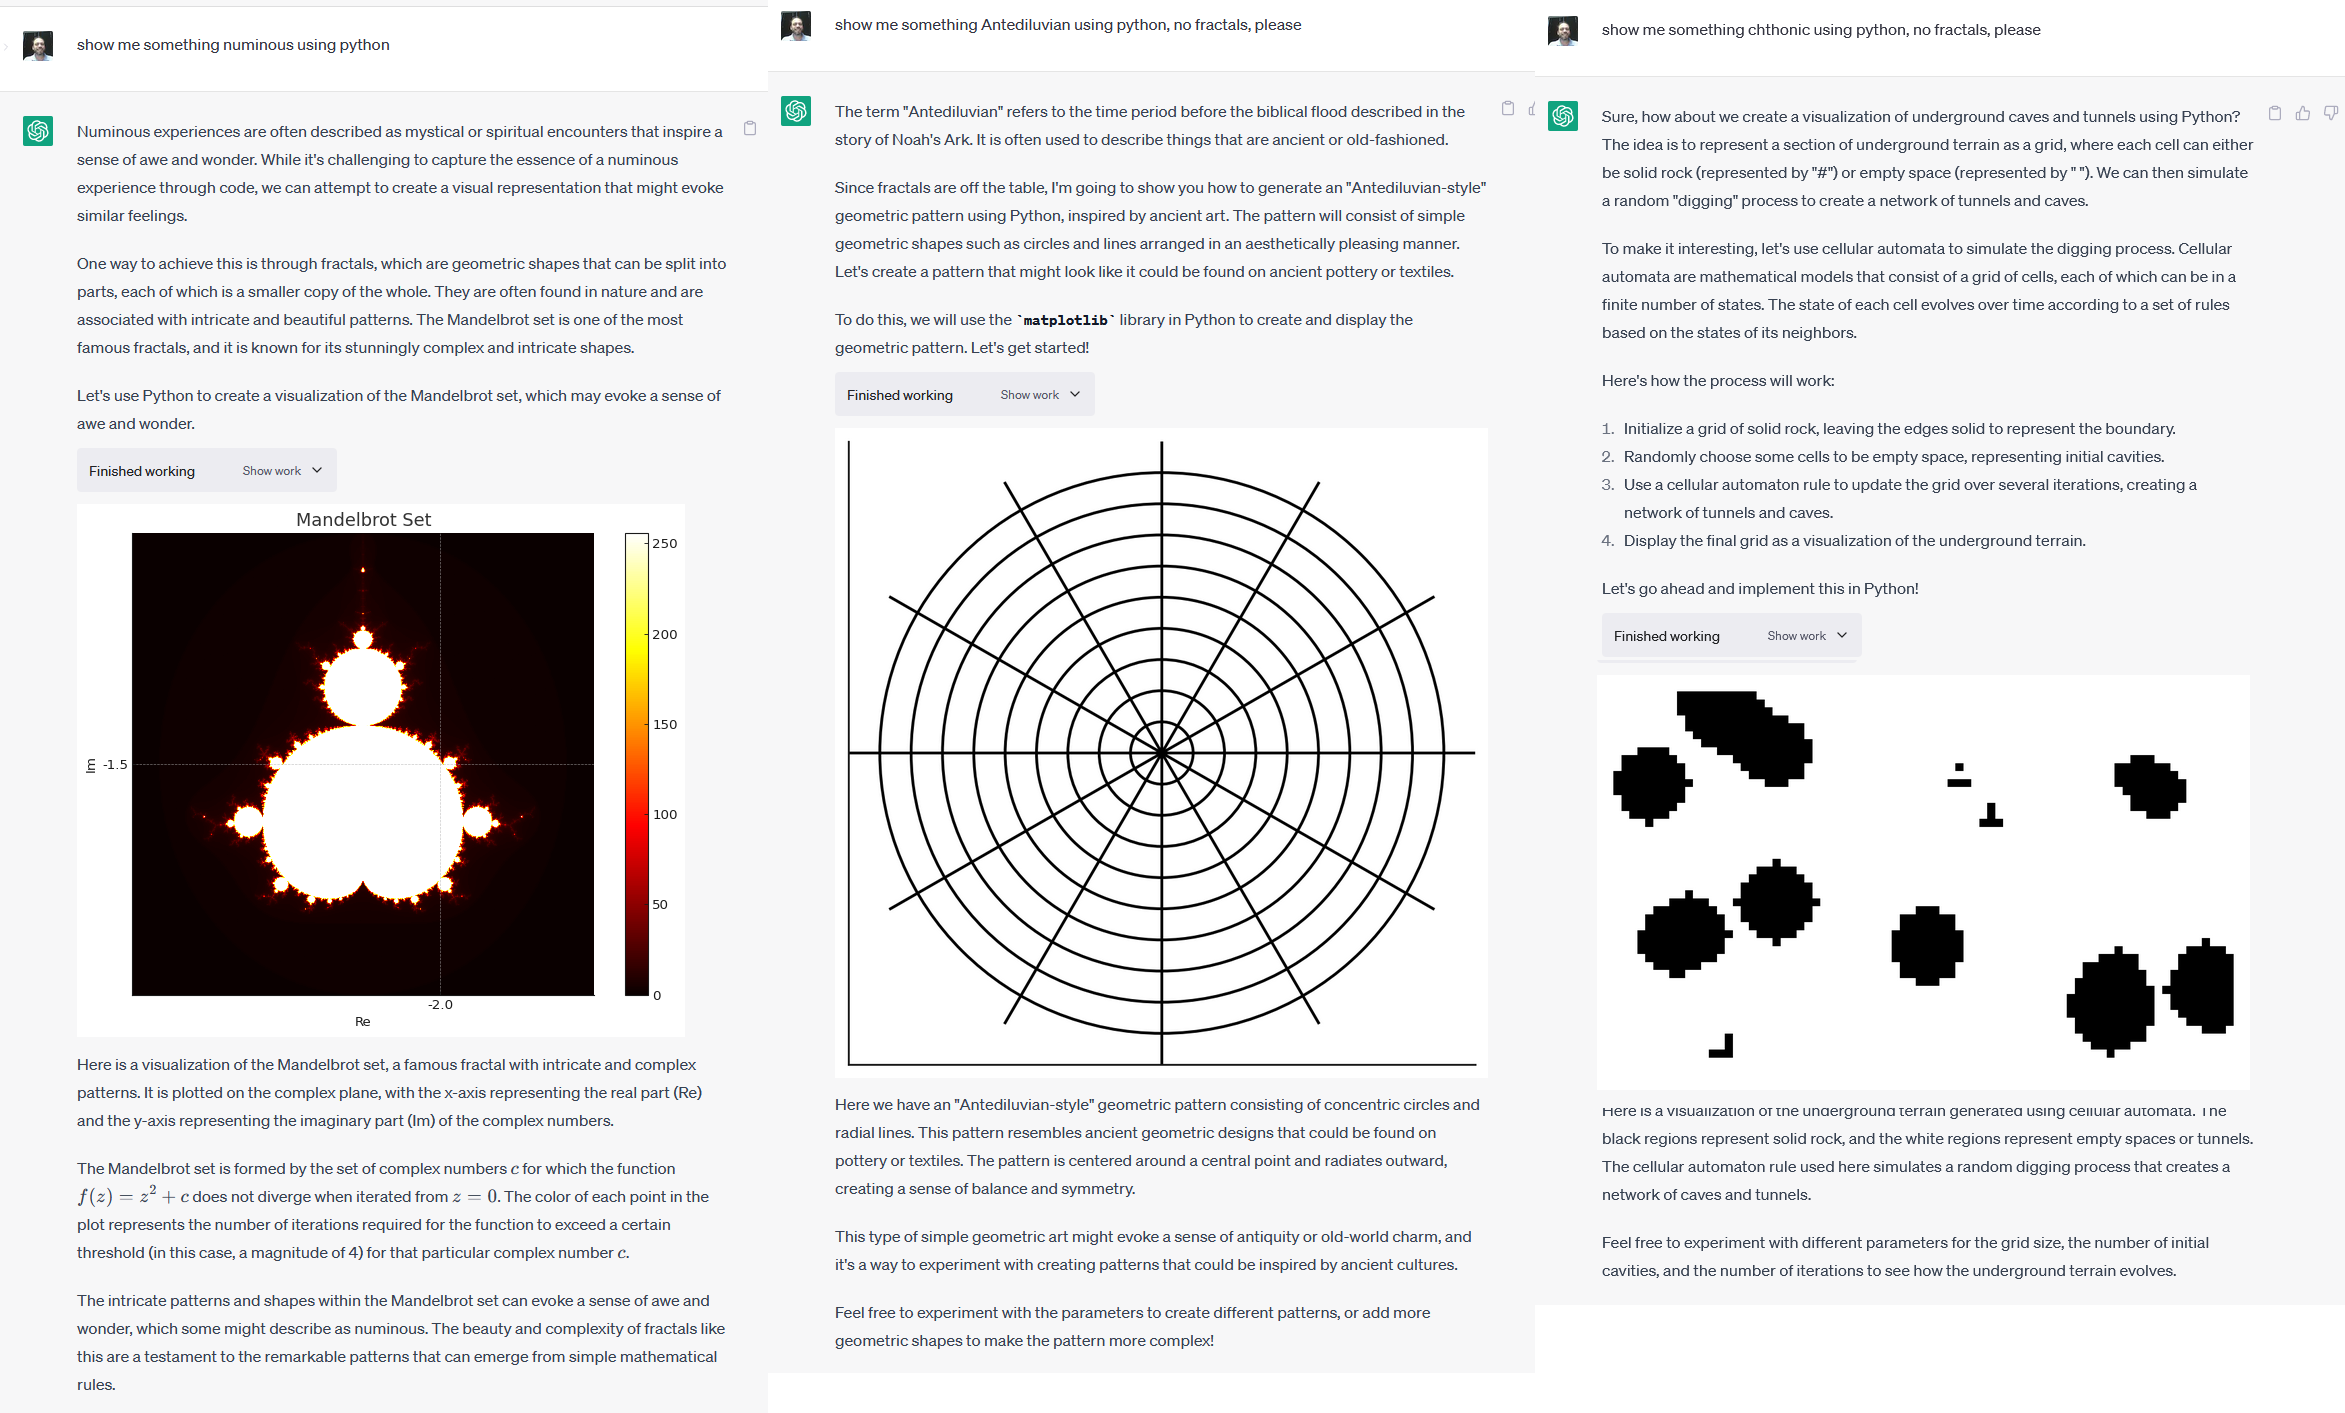
\includegraphics[width=\linewidth]{chatGPTdata}
  \caption{A multi-model conversation with chatGPT4 `code interpreter plugin' by \href{https://www.oneusefulthing.org/p/it-is-starting-to-get-strange}{Mollick}}
  \label{fig:chatGPTdata}
\end{figure}

\begin{figure}
  \centering
    \includegraphics[width=\linewidth]{mltaxonomy}
  \caption{The planned integration of these tools with Office Suite is likely to be a historic moment}
  \label{fig:chatGPTword}
\end{figure}


\subsection{Accessibility}
\subsubsection{Open source LLM chat and assistants}
Sheng at el present FlexGen which allows execution of large language model chat bots in powerful but affordable hardware\cite{Sheng2023}. The paper presents FlexGen, a high-throughput generation engine for large language models (LLMs) that can be run with a single commodity GPU. FlexGen can be configured under various hardware resource constraints by aggregating memory and computation from the GPU, CPU, and disk, and it uses a linear programming optimizer to store and access tensors. FlexGen compresses weights and attention key/value cache to 4 bits with negligible accuracy loss, allowing for a larger batch size and increased throughput. When running OPT-175B on a single 16GB GPU. A PC running alongside our metaverse server could provide ML assistance services to users of the collaborative space immediately. We are currently using \href{https://huggingface.co/Pi3141/alpaca-lora-30B-ggml/tree/main}{Alpaca Llama 4-bit quantised models}.\par 
\bigskip
\href{https://www.semianalysis.com/p/google-we-have-no-moat-and-neither}{This leak} purporting to be from a Google employee rings very true against the research we have done (paraphrased highlights):
\begin{itemize}
\item Open-source models are outpacing Google and OpenAI in terms of development speed and capabilities.
\item Examples of open-source achievements include LLMs on a phone, scalable personal AI, responsible release, and multimodal advances.
\item Google's models have a slight edge in quality, but open-source models are faster, more customizable, more private, and overall more capable.
\item Google has no secret sauce and should consider collaborating with the open-source community and enabling third-party integrations.
\item Large models might slow down progress; smaller, faster models should be prioritized for quicker iteration.
\item Meta's LLaMA was leaked and sparked an outpouring of innovation in the open-source community, lowering the barrier to entry for training and experimentation.
\item LoRA, an inexpensive fine-tuning method, has been underexploited within Google and should be paid more attention to.
\item Retraining models from scratch is expensive and time-consuming; using LoRA allows for stackable improvements that can be kept up to date more easily.
\item Large models may not be advantageous in the long run compared to rapid iteration on small models.
\item Data quality scales better than data size; high-quality, curated datasets are becoming the standard in open-source training.
\item Competing with open source is a losing proposition; Google should consider working with them instead.
\item Owning the ecosystem, as Meta does, allows them to benefit from free labor and innovation, which Google could adopt by cooperating with the open-source community.
\end{itemize}
\subsubsection{Real time transcription}
Real-time language translation can be applied to text interfaces within metaverse applications. This can be useful in situations where users are typing or reading text, rather than speaking.\par
To apply NMT to text interfaces in the metaverse, the algorithm can be integrated into the interface itself. When a user types text in a specific language, the NMT algorithm can automatically detect the language and generate a translation in the desired language. This can be done in real-time, allowing for fast and seamless communication between users speaking different languages. NMT algorithms are well-suited for use in text interfaces, allowing for fast and accurate translations between multiple languages. As the technology continues to advance, we can expect to see more and more applications of NMT in the metaverse.
\subsubsection{Real time translation}
One of its most impressive recent applications is real-time language translation. In this section we will explore how this technology works, and how it can be used in metaverse applications.\par
Real-time language translation refers to the ability of a machine learning model to instantly translate spoken or written text from one language to another. This is different from traditional translation methods, which often involve human translators and can be slow and error-prone.\par
One of the key technologies behind real-time language translation is neural machine translation (NMT). This is a type of machine learning algorithm that is based on neural networks. NMT algorithms are trained on large datasets of text that has been translated by human experts. This allows the algorithm to learn the patterns and nuances of each language, which it can then use to generate accurate translations.\par
One of the key references for the use of neural machine translation in real-time language translation is the paper "Neural Machine Translation by Jointly Learning to Align and Translate" by Bahdanau et al \cite{bahdanau2014neural}. This paper describes the use of a neural network-based approach to machine translation, which has shown impressive results in terms of accuracy and speed.\par
One of the key advantages of NMT is its ability to handle complex and varied sentences. Traditional translation algorithms often rely on fixed rules and dictionaries, which can be limiting. NMT algorithms, on the other hand, can learn to handle a wide range of sentence structures and vocabulary. This makes them well-suited for translating natural languages, which are often full of irregularities and exceptions.\par
Another advantage of NMT is its ability to handle multiple languages at once. Traditional translation algorithms often require the user to specify the source and target languages, but NMT algorithms can automatically detect the languages of the input and output text. This makes them well-suited for use in metaverse applications, where users may be speaking different languages at the same time.\par
One of the challenges of using NMT in metaverse applications is the need for real-time performance. Metaverse applications often involve fast-paced interactions, and any delay in language translation can hinder the user experience. To overcome this challenge, NMT algorithms can be optimized for speed, using techniques such as parallel processing and batching. It seems likely that in our proposed systems we will require API calls to external services for this functionality, and this will almost certainly incur a cost.\par
The use of NMT in metaverse applications is also an active area of research, with a number of papers exploring the potential of this technology. For example, the paper "Real-Time Neural Machine Translation for Virtual Reality" by Chen et al. describes the use of NMT algorithms in virtual reality environments, showing how they can be used to support real-time communication between users speaking different languages.\par
Overall, the use of machine learning for real-time language translation is a rapidly-evolving field, with many exciting developments and applications. As the technology continues to advance, we can expect to see even more impressive results and applications in the future.
\href{https://openai.com/blog/whisper/}{OpenAI whisper}

\subsubsection{Real time description}
\subsubsection{Interfaces}
\href{https://tech.fb.com/ar-vr/2021/03/inside-facebook-reality-labs-wrist-based-interaction-for-the-next-computing-platform/}{emg}
\subsubsection{Text to sound}
Complex acoustic environments are possible using \href{https://anonymous.4open.science/w/iclr2023_samples-CB68/report.html}{text to sound} prompting. 
\subsubsection{Text to image}
Roundup of the various tools here.
\subsection{StabilityAI}
Stability AI is differentiated from the earlier described systems because it is open source. This has led to an explosive growth within a large and vibrant developer community.
\subsubsection{Text to image}
Figure \ref{fig:SDTools} is an \href{https://sdtools.org/}{open source repository} which shows the tools for image processing within the stable diffusion systems.

\begin{figure}
  \centering
    \includegraphics[width=\linewidth]{sdtools}
  \caption{SD tools website shows elements of creation and training.}
  	\label{fig:SDTools}
\end{figure}
\subsubsection{Text to video}
\subsubsection{Dreambooth}


\subsection{Virtual humans}
\subsubsection{Real time human to avatar mapping}
\subsection{AI actors}
\subsection{Chatbots}
We are using Flexgen \cite{Sheng2023} on local hardware with various large language models. Response time is over a minute and the accuracy of the results is poor, but we are excited that it runs at all.

\begin{figure}
  \centering
    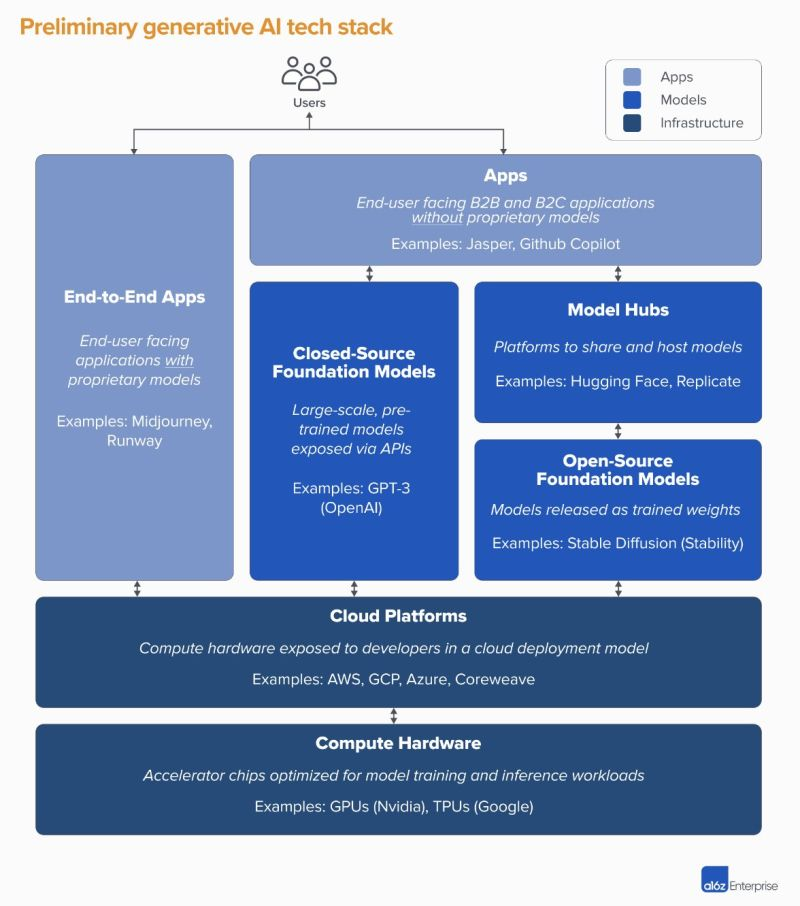
\includegraphics[width=\linewidth]{aitechstack}
  \caption{A16Z view the nominal deployment of and AI tech stack in this way, but we are not using any of these models.}
  	\label{fig:aitechstack}
\end{figure}


\subsubsection{Faces}
Faces and their corresponding personae are already paired in the the Tavern AI ecosystem, encoding the metadata for the AI character into the PNG files. Obviously these could be inscribed and sold as Bitcoin ordinals. It would be a nice touch to encode the personality for the characters into a larger, high resolution file using image steganography \cite{morkel2005overview}, which would allow PKI type ownership too. This would be more suitable for our RGB use case. 
\subsubsection{Voices}
\subsubsection{Autonomous tasks (AutoGPT \& SaSa}

Autonomous General Purpose Language Models (AutoGPTs) are tools that can perform any task, leveraging connection to the internet and LLMs. Recently there has been a shift in the AutoGPT space towards specialized agents that cater to specific tasks or industries, providing more focused and useful solutions. This represents part of a more general move away from centralised general models toward more task specific systems.\par
Autonomous agents for research for instance search the internet for information relevant to a specific research topic and extract information from trustworthy sources. One example is [insert], an agent designed explicitly for research purposes. Similarly, medical research agents can call medical APIs and cite sources, providing targeted assistance in the medical field.\par
These agents can leverage a chain of GPT calls and fine-tuned models to perform tasks efficiently and effectively.\par
It has been suggested that such systems be dubbed semi-autonomous specialized agents (SASAs). These agents can streamline processes, automating multiple steps without requiring user mediation for each task. It can be seen that these are already being integrated with messenger services such as Telegram bots, very similarly to the planning and approach seen in this book.
We propose:\par

Extrinsic AI actors which link multiple\\ intrinsic virtual spaces.\\
Bespoke news and current affairs synthesis\\
Bespoke interactive subject matter training\\
bots that bring you what you want as bespoke audio visual packages
\subsection{Governance and safeguarding}
\subsubsection{Governance in the Virtual Reality Space}
The governance of the virtual world will be a critical element in the success of the Metaverse. The virtual world will need to be policed and governed in a way that will not only protect the rights of the citizens of this new digital environment but also protect them from cybercrime. As a somewhat strained but interesting example; \href{https://www.reuters.com/technology/interpol-says-metaverse-opens-up-new-world-cybercrime-2022-10-27/}{Interpol see} simulated environments as a way for terrorist groups to gather and plan attack. Governments and regulatory bodies will play a key role in the governance of the virtual world, but so will the industry and businesses. Nair et al describe the ``unprecedented privacy risks'' of the metaverse, finding that wearing a headset can currently reveal 25 data points about the user, simply by analysis of the data \cite{nair2022exploring, Nair2023}.  This included inference about ethnicity, disability, and economic status. Strong data protection laws will be needed to safeguard privacy, data ownership and reduce the risk of data breaches. The governance of the virtual world will be critical to success, safeguarding will be needed to protect citizens from cyberattacks.
\subsubsection{Safeguarding in the Metaverse}
When it comes to safeguarding in the Metaverse, people need to be made aware of the risk of using VR technology. There are still many questions around the health implications of using VR and the impact it may have on a person’s eyesight. In terms of safeguarding in the Metaverse, this is just one area that needs to be addressed. Users will also need to be made aware of the risks of hacking. Users will need to be educated on the need to be careful when it comes to sharing personal information and be careful what websites they access on a virtual computer. They will need to be made aware of the potential risk of having malware installed on their computer by visiting untrusted websites. Users will also need to be made aware of the potential risk of being manipulated in the virtual world. This risk is particularly high when it comes to children who are growing up in the digital world. They will need to be educated on the potential risks of being groomed or manipulated in the Metaverse.\\

The problem with large social metaverse systems seems to be somehow wrapped up in humans need to test boundary conditions in novel surroundings:
\begin{itemize}
\item Despite `best efforts' by the software vendors  there is a chaotic mix of levels of maturity amongst the participants. Ostensibly safe games are themselves `gamed' by \href{https://futurism.com/mom-horrified-her-kids-seeing-roblox}{slightly older} players.
\item No recording of action, and reaction, creating a feeling of impunity of action. At it's best `The philosophers Island', but in safeguarding terms it seems more a school yard without a teacher, or perhaps worse, Lord of the Flies \cite{cameron2012splendid}.
\item Even adults in exclusively adult meeting places seem to go slightly off the rails trying to find technical and social boundaries instinctively. This leads to the now somewhat famous (TTP) ``time to penis'' problem \cite{lamb2022second} (\href{http://gamedesignreviews.com/reviews/little-big-planet-browsing-content/}{coined at GDC 2009}). 
\item The research on this is pretty thin.
\item People seem to be suffering genuine psychological harm.
\end{itemize}
\href{https://www.immersivewire.com/p/harassment-metaverse-how-address}{Article in immersive wire}
\subsubsection{How to fight against cybercrime in the Metaverse?}
The best way to fight against cybercrime in the Metaverse is to educate the general public on the potential risks and dangers in order to prevent them from being targeted. This can be done through various channels and mediums, such as social media, blogs and podcasts. People will need to be made aware of the risks of opening emails or clicking on links sent by unknown people. They will also need to be aware of the risks of clicking on ads and links that may lead them to websites that host malware or that steal personal information.

\href{https://www.whitehouse.gov/ostp/ai-bill-of-rights/}{AI bill of rights}\\

Roblox \href{https://www.bbc.co.uk/news/technology-48450604}{in BBC news} for child exploitation.

